\documentclass[10pt,xcolor=table,aspectratio=169]{beamer}

\usepackage{graphicx}
\usepackage{caption}
\usepackage{subcaption}
\usepackage{transparent}
\usepackage{epstopdf} %converting to PDF
\usepackage{multicol} 
\usepackage{animate}[2017/05/18]
% \usepackage{subfig}

\usepackage{makecell}

% \usepackage{pdfx}
 
% \usepackage[utf8]{inputenc}
% \usepackage[T1]{fontenc}
\usepackage[table]{xcolor}    % loads also »colortbl« 
%  \usepackage{enumitem}
% \usepackage{ucltemplate}
\usepackage{color}

\usepackage{comment}

\usepackage{tabularx} % make width of table columns evenly distributed (see http://tex.stackexchange.com/questions/60601/evenly-distributing-column-widths)
% \newcolumntype{Y}{>{\centering\arraybackslash}X}

% make entire row bold or italic in table
\newcommand\setrow[1]{\gdef\rowmac{#1}#1\ignorespaces}
\newcommand\clearrow{\global\let\rowmac\relax}
\clearrow


\usepackage{amssymb}% http://ctan.org/pkg/amssymb
\usepackage{pifont}% http://ctan.org/pkg/pifont
\newcommand{\cmark}{\ding{51}}%
\newcommand{\xmark}{\ding{55}}%


%\usepackage{pgfgantt} % for grantt charts
\usepackage{rotating}
\usepackage[graphicx]{realboxes}
\usepackage[export]{adjustbox}
\usepackage{array}

\usepackage{rotating}
% \usepackage{tabularx, booktabs} % make width of table columns evenly distributed (see http://tex.stackexchange.com/questions/60601/evenly-distributing-column-widths)
% \newcolumntype{Y}{>{\centering\arraybackslash}X}

\DeclareMathOperator*{\argmin}{arg\,min}
\DeclareMathOperator*{\argmax}{arg\,max}

\usepackage{tikz}
\usetikzlibrary{arrows,positioning, shapes.symbols,shapes.callouts,patterns,shapes,chains,calc,backgrounds,fadings}

% \definecolor{parCol}{rgb}{0.1, 0.1, 1}
% \definecolor{stCol}{rgb}{0.1, 0.6, 0.1}
% \definecolor{bothCol}{rgb}{0, 0.5, 0.5}

\definecolor{parCol}{rgb}{0, 0, 0}
\definecolor{stCol}{rgb}{0, 0, 0}
\definecolor{bothCol}{rgb}{0, 0, 0}
\definecolor{blue3}{HTML}{86B7FC} % med blue
\definecolor{blue1}{HTML}{B5F1FF} % light blue
\definecolor{blue2}{HTML}{E0F9FF} % very light blue

\newcolumntype{C}[1]{>{\centering\let\newline\\\arraybackslash\hspace{0pt}}m{#1}}

\setlength{\tabcolsep}{0.2em}

 
 %% OVERVIEW OF WORK SO FAR %%
 
%Information to be included in the title page:
\title{BrainPainter: A software for the visualisation of brain structures, biomarkers and associated pathological processes}
\author[Raz]{\footnotesize{R\u{a}zvan V. Marinescu\inst{1,2} \and Arman Eshaghi\inst{2} \and Daniel C. Alexander\inst{2} \and Polina Golland\inst{1}}}



\institute{
1. Computer Science and Artificial Intelligence Laboratory, MIT, Cambridge, USA\\
% \and
2. Centre for Medical Image Computing, UCL, London, UK\\
3. Queen Square MS Centre, UCL Institute of Neurology, London, UK\\
}


\vspace{0em}
% \small{Centre for Medical Image Computing, University College London, UK}
% }

\date{}

\newcommand{\heightLogo}{0.8cm}

% logo of my university
\titlegraphic{
    \vspace{-2em}
%     \begin{figure}
%     \includegraphics[height=1.cm]{tadpole_logo}
%     \end{figure}


   \begin{figure}
   \begin{subfigure}{0.32\textwidth}
   \centering
%    2.\\
   
\includegraphics[height=\heightLogo]{images/MIT_logo}
   \end{subfigure}
   \begin{subfigure}{0.32\textwidth}
   \hspace{2.5em}
    \centering
%    1.\\
   
\includegraphics[height=\heightLogo, trim=70 0 0 10, clip]{images/ucl_logo}
   \end{subfigure}
   \end{figure}

%    \vspace{1em}
%    \tiny{Slides available online: https://people.csail.mit.edu/razvan/talk/tadpoleMICCAI/tadpole\_pres.pdf}
}

\setbeamercolor{frametitle}{fg=black}
\setbeamercolor{author in head/foot}{fg=black, bg=white} 
\setbeamercolor{institute in head/foot}{fg=black, bg=white} 
\setbeamercolor{title in head/foot}{fg=black, bg=white}
\setbeamercolor{date in head/foot}{fg=black, bg=white}

\setbeamersize{text margin left=10pt,text margin right=10pt}
% \setbeamertemplate{frametitle}{
%     \vspace{0.9em}
%     \insertframetitle
% %     \vspace{-3em}
% }
\setbeamertemplate{frametitle}{%
    \vspace{0.5em}
    \usebeamerfont{frametitle}\insertframetitle%
    \vphantom{g}% To avoid fluctuations per frame
    %\hrule% Uncomment to see desired effect, without a full-width hrule
    \par% <-- added
    \hspace*{-\dimexpr0.5\paperwidth-0.5\textwidth}% <-- calculation of left margin width
    \rule[0.5\baselineskip]{\paperwidth}{0.4pt}%
}

\setbeamertemplate{footline}
{
  \vspace{-3em}
  \leavevmode%
   \rule{\paperwidth}{0.3pt}
  \hbox{%
  \begin{beamercolorbox}[wd=.2\paperwidth,ht=2.25ex,dp=1ex,center]{author in head/foot}%
    \usebeamerfont{author in head/foot}Razvan Marinescu
  \end{beamercolorbox}%
  \begin{beamercolorbox}[wd=.2\paperwidth,ht=2.25ex,dp=1ex,center]{institute in head/foot}%
    \usebeamerfont{institute in head/foot}BrainPainter
  \end{beamercolorbox}%
  \begin{beamercolorbox}[wd=.3\paperwidth,ht=2.25ex,dp=1ex,center]{institute in head/foot}%
    \usebeamerfont{institute in head/foot}https://brainpainter.csail.mit.edu/
  \end{beamercolorbox}%
  \begin{beamercolorbox}[wd=.2\paperwidth,ht=2.25ex,dp=1ex,center]{title in head/foot}%
    \usebeamerfont{title in head/foot}\insertsection
  \end{beamercolorbox}%
  \begin{beamercolorbox}[wd=.10\paperwidth,ht=2.25ex,dp=1ex,right]{date in head/foot}%
    \usebeamerfont{date in head/foot}\insertshortdate{}\hspace*{2em}
    \insertframenumber{} / \inserttotalframenumber\hspace*{2ex}
  \end{beamercolorbox}}%
  \vskip0pt%
}

% \usepackage{beamerthemesplit}

\newcommand{\backupbegin}{
   \newcounter{finalframe}
   \setcounter{finalframe}{\value{framenumber}}
}
\newcommand{\backupend}{
   \setcounter{framenumber}{\value{finalframe}}
}


\makeatletter
\long\def\beamer@author[#1]#2{%
  \def\and{\tabularnewline}
  \def\insertauthor{\def\inst{\beamer@insttitle}\def\and{\tabularnewline}%
  \begin{tabular}{rl}#2\end{tabular}}%
  \def\beamer@shortauthor{#1}%
  \ifbeamer@autopdfinfo%
    \def\beamer@andstripped{}%
    \beamer@stripands#1 \and\relax
    {\let\inst=\@gobble\let\thanks=\@gobble\def\and{, }\hypersetup{pdfauthor={\beamer@andstripped}}}
  \fi%
}
\makeatother
\beamertemplatenavigationsymbolsempty
\setbeamertemplate{caption}[numbered]
\setbeamercolor{caption name}{fg=black}
\setbeamercolor{itemize item}{fg=black}
\setbeamercolor{itemize subitem}{fg=black}
\setbeamercolor{enumerate item}{fg=black}
\setbeamercolor{enumerate subitem}{fg=black}
\setbeamertemplate{enumerate item}[default]
\setbeamertemplate{enumerate subitem}

\setbeamertemplate{itemize item}[circle]
\setbeamertemplate{itemize subitem}[circle]
% \setbeamertemplate{itemize subsubitem}[default]

% \renewcommand\labelitemi{---}

\makeatletter
\let\@@magyar@captionfix\relax
\makeatother
\begin{document}
 
\section{Introduction}

 \frame{\titlepage}
 
\setbeamerfont{frametitle}{size=\large}

\newcommand{\upgradeReportLoc}{../../upgrade_report}
\newcommand{\epsrcPresLoc}{\upgradeReportLoc/epsrcPres}
\newcommand{\jointModellingDiseaseLoc}{../../jointModellingDisease}
\newcommand{\pcaLongPaperLoc}{../../PCA_long_paper}
\newcommand{\voxFld}{../../voxelwiseDPM}
\newcommand{\tadpoleFld}{/research/tadpole}
\newcommand{\diffEqModelFld}{../../diffEqModel}



\newcommand*{\pcaLongFigs}{\pcaLongPaperLoc/figures}






\newcommand{\ovHeight}{2cm}

% 
% % % TODO continue with overview, move into commands
% \newcommand{\ovEBM}{
% \begin{subfigure}{0.47\textwidth}
% \centering
% 1. Modelled progression of PCA and tAD\\
% (using existing methods)
% \includegraphics[height=\ovHeight]{ebm_thumb.png}
% \end{subfigure}
% }
% 
% \newcommand{\ovVWDPM}{
% \begin{subfigure}{0.47\textwidth}
% \centering
% % \vspace{2.8em}
% 2. Developed Novel Spatio-temporal Model \\ (DIVE)\\
% \includegraphics[height=\ovHeight]{\upgradeReportLoc/images/vwdpm/blend14_adniThavgFWHM0InithistCl3Pr0Ra1_VWDPMStd.png}
% \end{subfigure}
% }
% 
% 
% \newcommand{\ovDKT}{
% \begin{subfigure}{0.47\textwidth}
% \centering
% \vspace{2em}
% 3. Developed Novel Transfer Learning \\ method (DKT) \\
% \vspace{0.5em}
% \includegraphics[height=2.2cm]{\jointModellingDiseaseLoc/paper/figures/disease_knowledge_transfer.pdf}
% \end{subfigure}
% }
% 
% 
% \newcommand{\ovTadpole}{
% \begin{subfigure}{0.47\textwidth}
% \centering
% \vspace{-2em}
% 4. Organised TADPOLE Competition\\
% \vspace{1em}
% \includegraphics[height=1.2cm,valign=t]{\upgradeReportLoc/epsrcPres/tadpole} 
% \end{subfigure}
% }
% 
% \newcommand{\ovPainter}{
% \begin{subfigure}{\textwidth}
% \centering
% \vspace{0.5em}
% 5. Created BrainPainter software\\
% 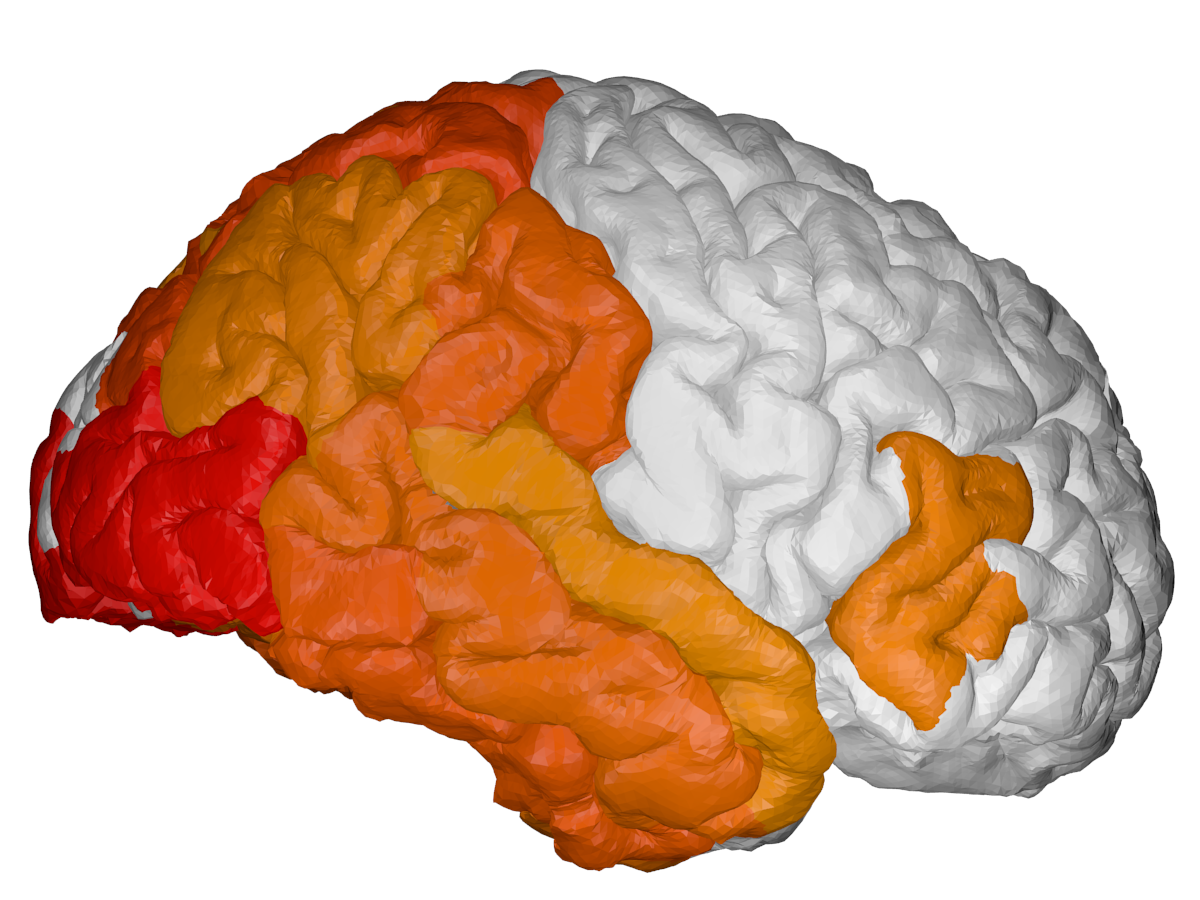
\includegraphics[height=1.5cm]{cortical-front_1}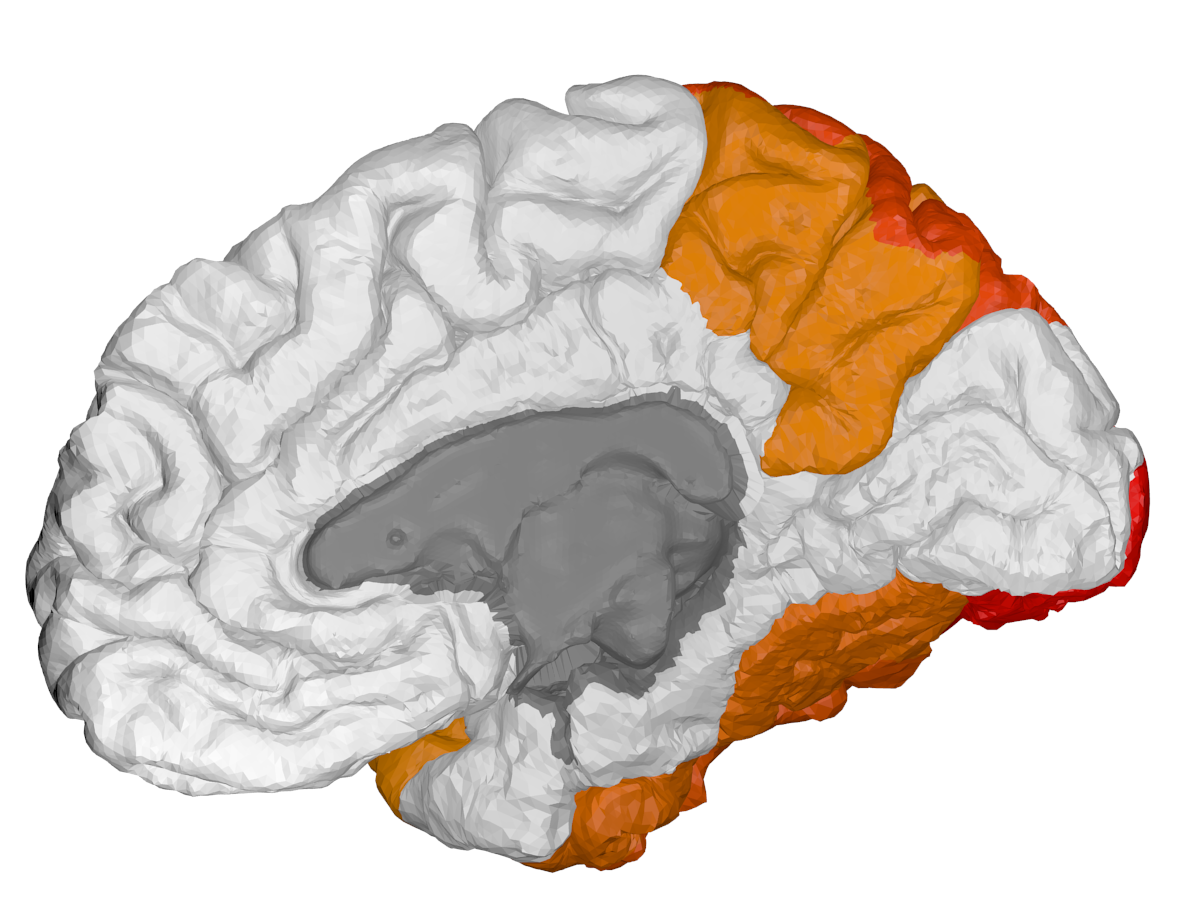
\includegraphics[height=1.5cm]{cortical-back_1}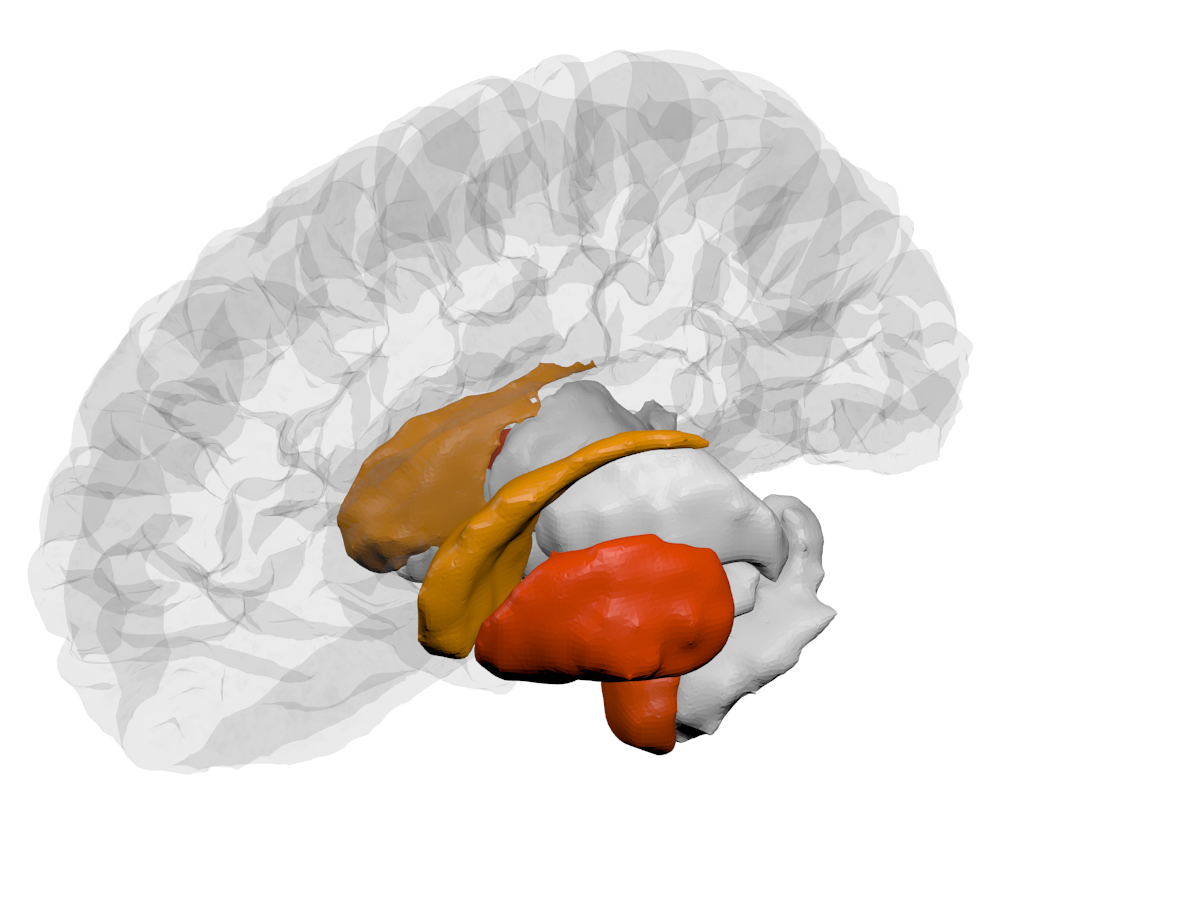
\includegraphics[height=1.5cm]{subcortical_1}
% \end{subfigure}
% }


\definecolor{light-gray}{gray}{0.6}



% Story: motivation, problems with current neuroimaging software (FS, slicer). 
% Need to perform animations
% 

\begin{frame}[t]
 \frametitle{Current brain visualisation software has several limitations}

 \definecolor{green1}{rgb}{0, 0.6, 0}
\definecolor{red1}{rgb}{0.9, 0, 0}
% \newcommand{\xmark}{\ding{55}}%

 
\newcommand{\myyes}{\textcolor{green1}{\Large{\textbf{\checkmark}}}}
\newcommand{\myno}{\textcolor{red1}{\Large{\xmark}}}

%  \vspace{-0.5cm}
\begin{figure}
\centering
\begin{subfigure}[t]{0.3\textwidth}
\centering
 \begin{minipage}[t][3.5cm][t]{\textwidth}
 \centering
\myno requires specialised input files\\

\includegraphics[width=0.5\textwidth]{images/inputFile} 
 \end{minipage}


% \myyes generic and simple input files
% 
% \begin{itemize}
%  \item generated by e.g. spreadsheet
%  \item list of colours, one for each ROI
% \end{itemize}


% \begin{table}
% \centering
%  \fontsize{7}{8}\selectfont
% \begin{tabular}{c | c c c}
%  Biomarkers &  Hippocampus & Inferior & ...\\
%  &              & temporal & ...\\
%   \hline
% % Brain 1 & 0.6 & 2.3 & .. \\
% % Brain 2 & 1.2 & 0.0 & .. \\
% ... & \multicolumn{3}{c}{...}\\
% \end{tabular}
% \end{table}

\end{subfigure}
\begin{subfigure}[t]{0.3\textwidth}
\centering
 \begin{minipage}[t][3.5cm][t]{\textwidth}
 \centering
\myno cannot automate image generation\\
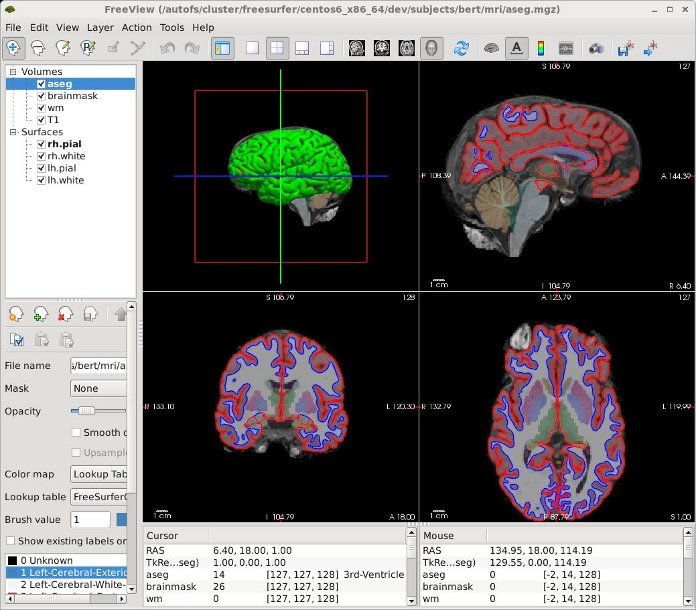
\includegraphics[width=0.5\textwidth]{images/freeviewInterface.jpg}
 \end{minipage}


% \myyes can be used to generate multiple images
% 
% 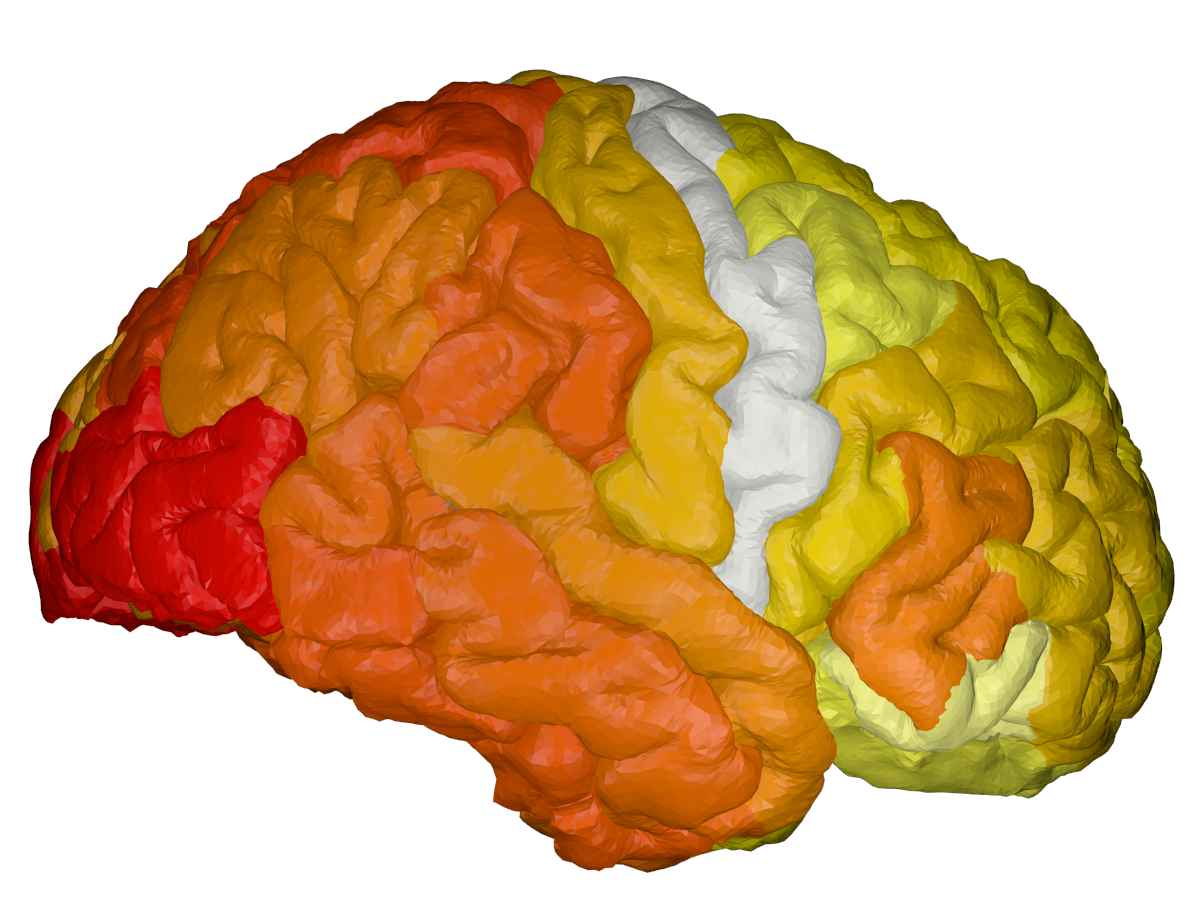
\includegraphics[height=1cm,trim=0 0 900 0]{images/brainTransparent} 
% 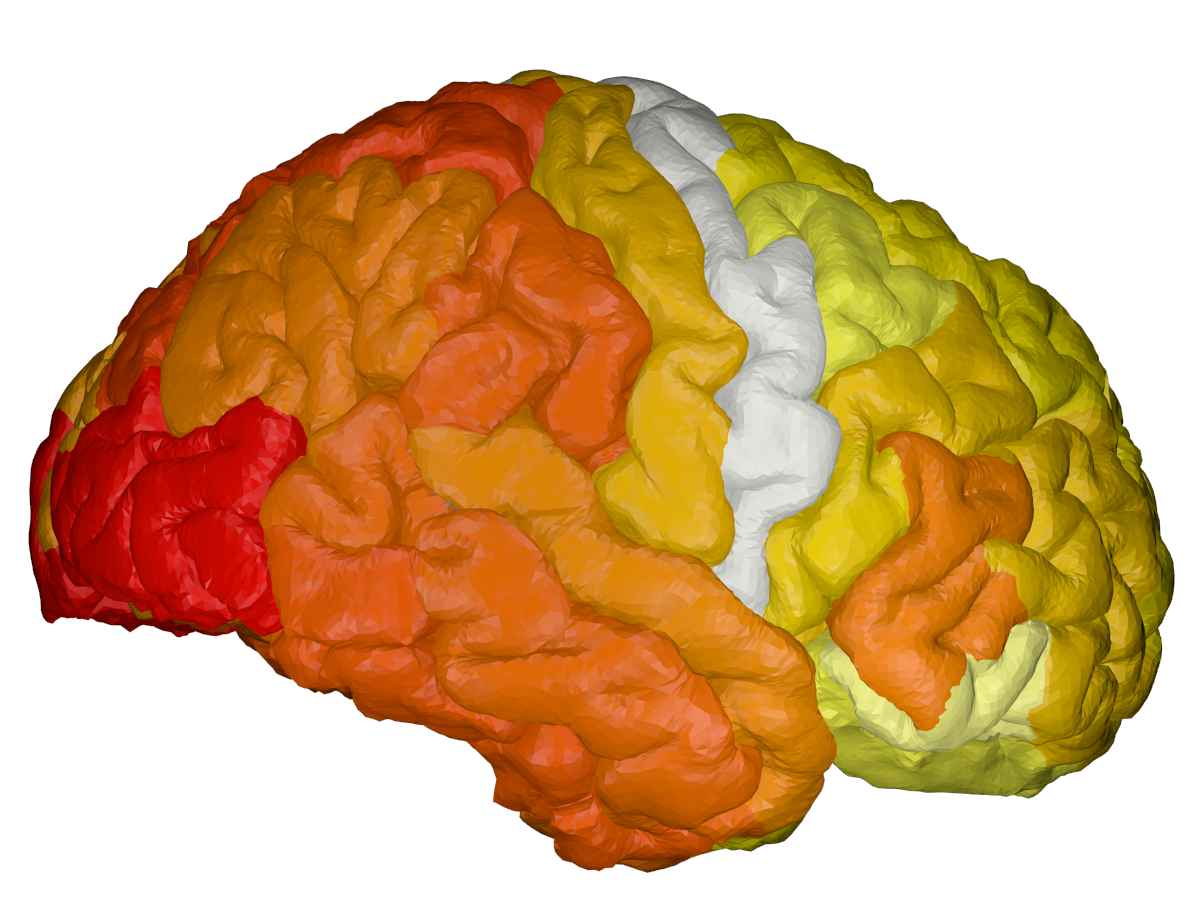
\includegraphics[height=1cm,trim=0 0 900 0]{images/brainTransparent} 
% 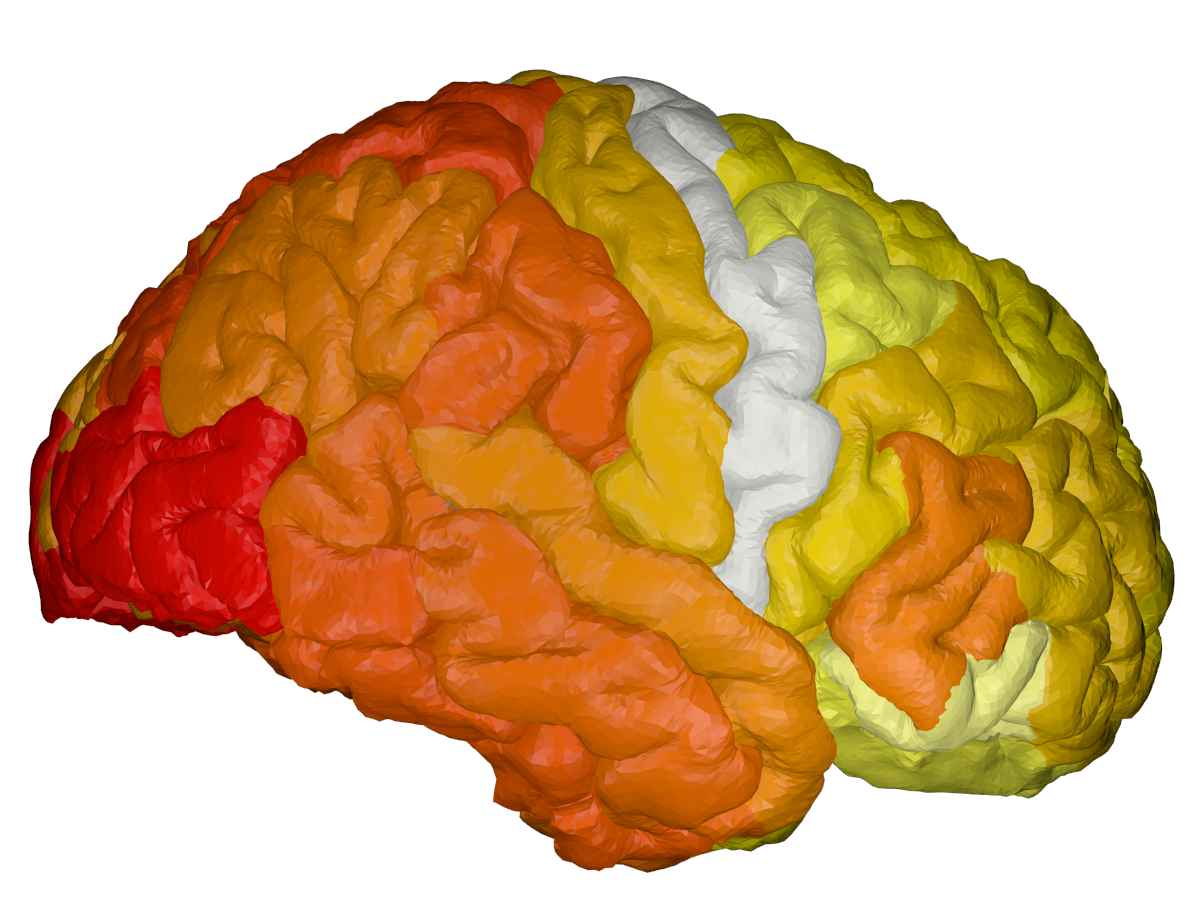
\includegraphics[height=1cm,trim=0 0 900 0]{images/brainTransparent} 
% 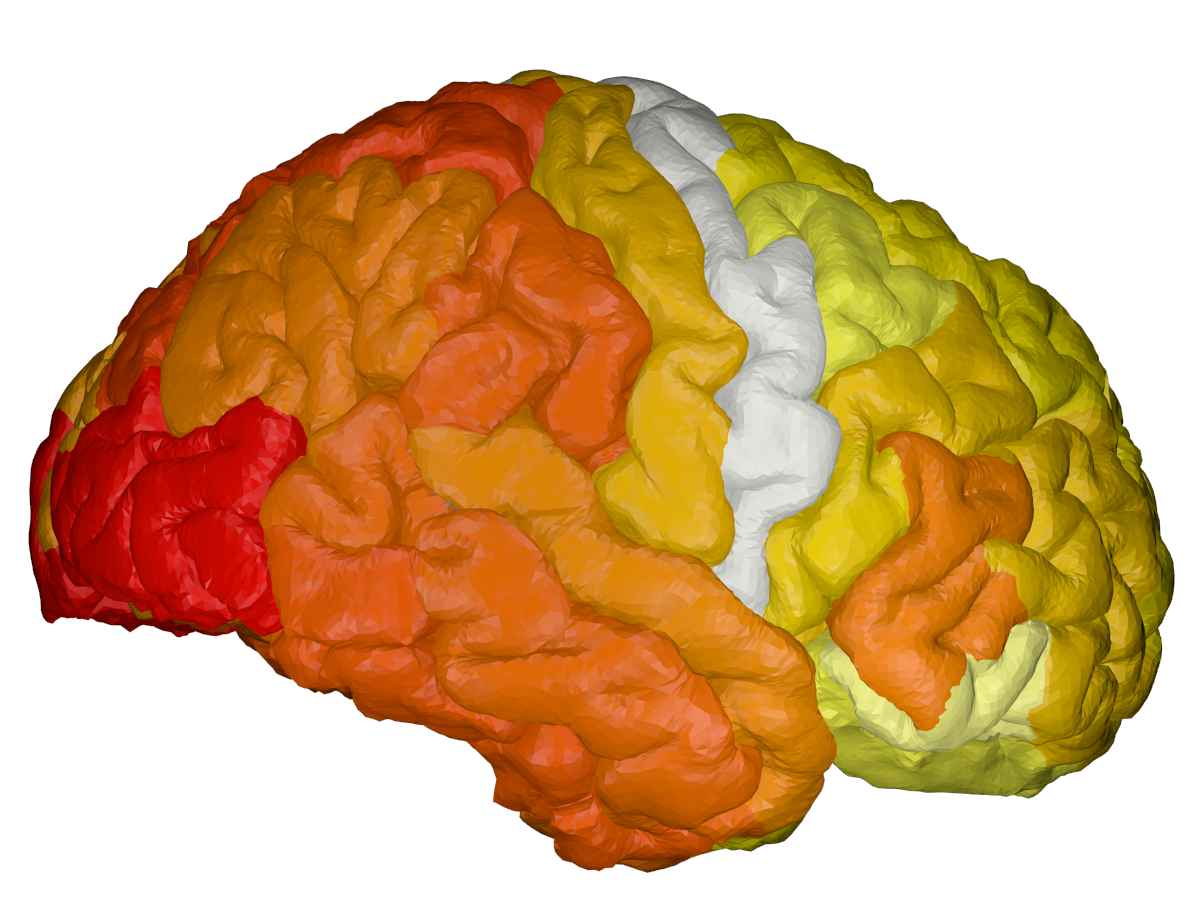
\includegraphics[height=1cm]{images/brainTransparent} 



\end{subfigure}
\begin{subfigure}[t]{0.3\textwidth}
\centering
 \begin{minipage}[t][3.5cm][t]{\textwidth}
 \centering
\myno volumetric images hard to visualise\\
\vspace{1.5em}
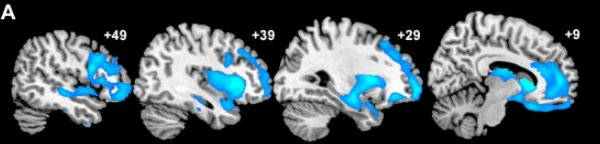
\includegraphics[width=\textwidth]{images/seeleyImages} 
\vspace{1.0em}
 \end{minipage}


% \myyes brain surface easy to visualise\\
% 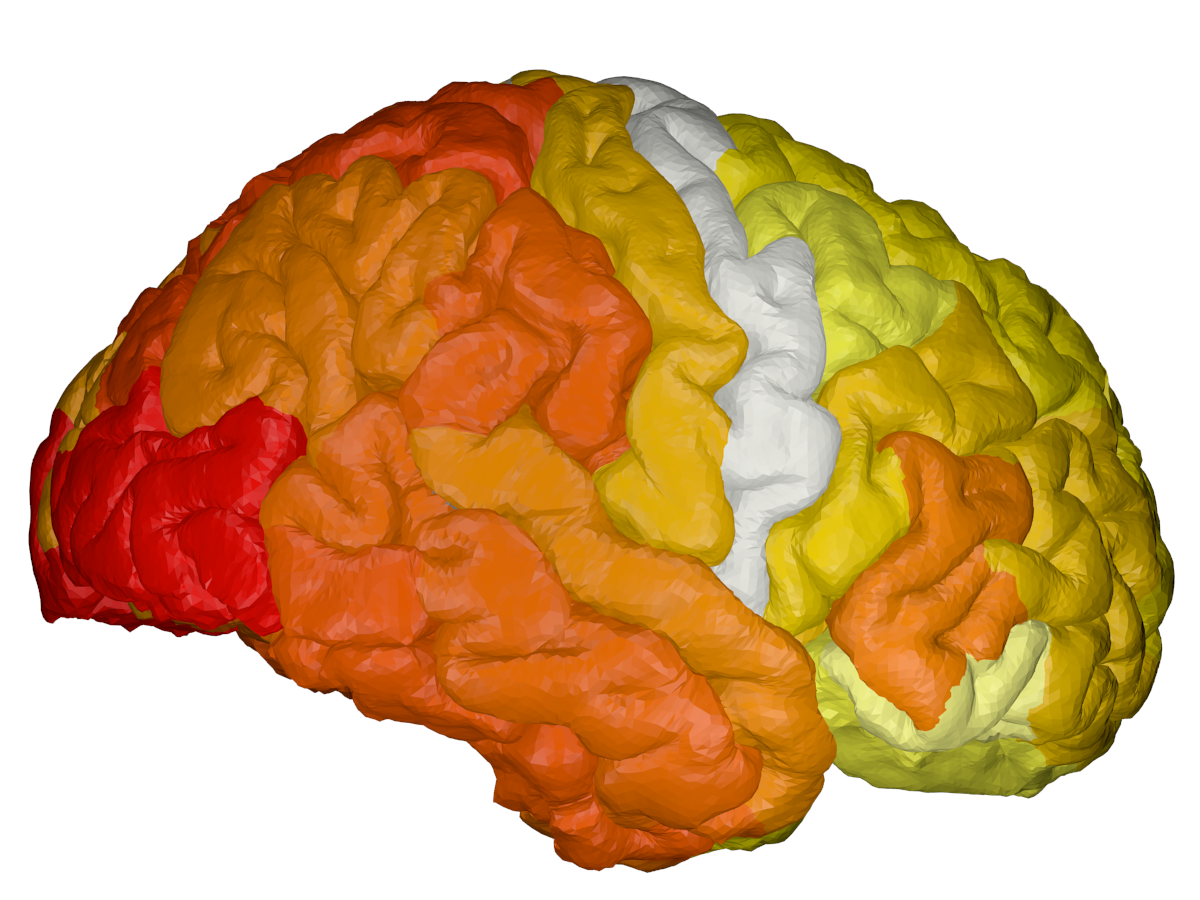
\includegraphics[width=0.5\textwidth]{images/cortical-outer_0} 


\end{subfigure}

\end{figure}
 
\end{frame}


\begin{frame}[t]
 \frametitle{Aim: Develop a brain visualisation software that overcomes such limitations}

 \definecolor{green1}{rgb}{0, 0.6, 0}
\definecolor{red1}{rgb}{0.9, 0, 0}
% \newcommand{\xmark}{\ding{55}}%

 
\newcommand{\myyes}{\textcolor{green1}{\Large{\textbf{\checkmark}}}}
\newcommand{\myno}{\textcolor{red1}{\Large{\xmark}}}

%  \vspace{-0.5cm}
\begin{figure}
\centering
\begin{subfigure}[t]{0.3\textwidth}
\centering
 \begin{minipage}[t][3.5cm][t]{\textwidth}
 \centering
\myno requires specialised input files\\

\includegraphics[width=0.5\textwidth]{images/inputFile} 
 \end{minipage}


\myyes generic and simple input files

\begin{itemize}
 \item generated by e.g. spreadsheet
 \item list of colours, one for each ROI
\end{itemize}


% \begin{table}
% \centering
%  \fontsize{7}{8}\selectfont
% \begin{tabular}{c | c c c}
%  Biomarkers &  Hippocampus & Inferior & ...\\
%  &              & temporal & ...\\
%   \hline
% % Brain 1 & 0.6 & 2.3 & .. \\
% % Brain 2 & 1.2 & 0.0 & .. \\
% ... & \multicolumn{3}{c}{...}\\
% \end{tabular}
% \end{table}

\end{subfigure}
\begin{subfigure}[t]{0.3\textwidth}
\centering
 \begin{minipage}[t][3.5cm][t]{\textwidth}
 \centering
\myno cannot be automated for image generation\\
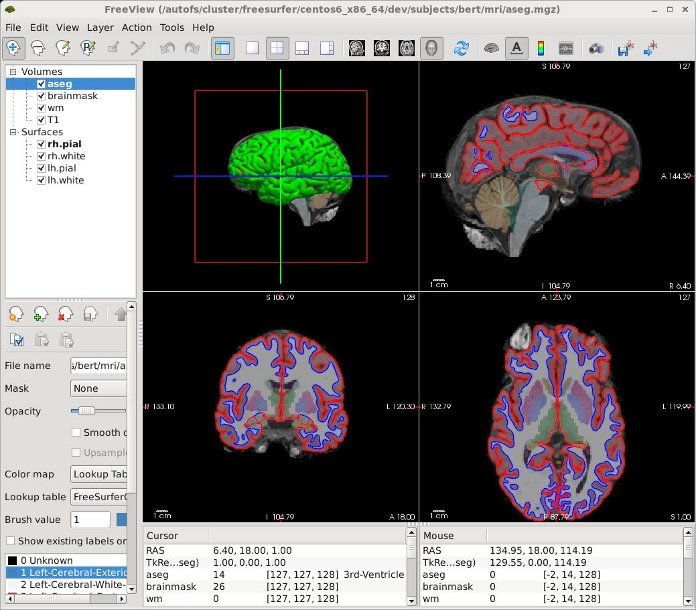
\includegraphics[width=0.5\textwidth]{images/freeviewInterface.jpg}
 \end{minipage}


\myyes can automate image generation

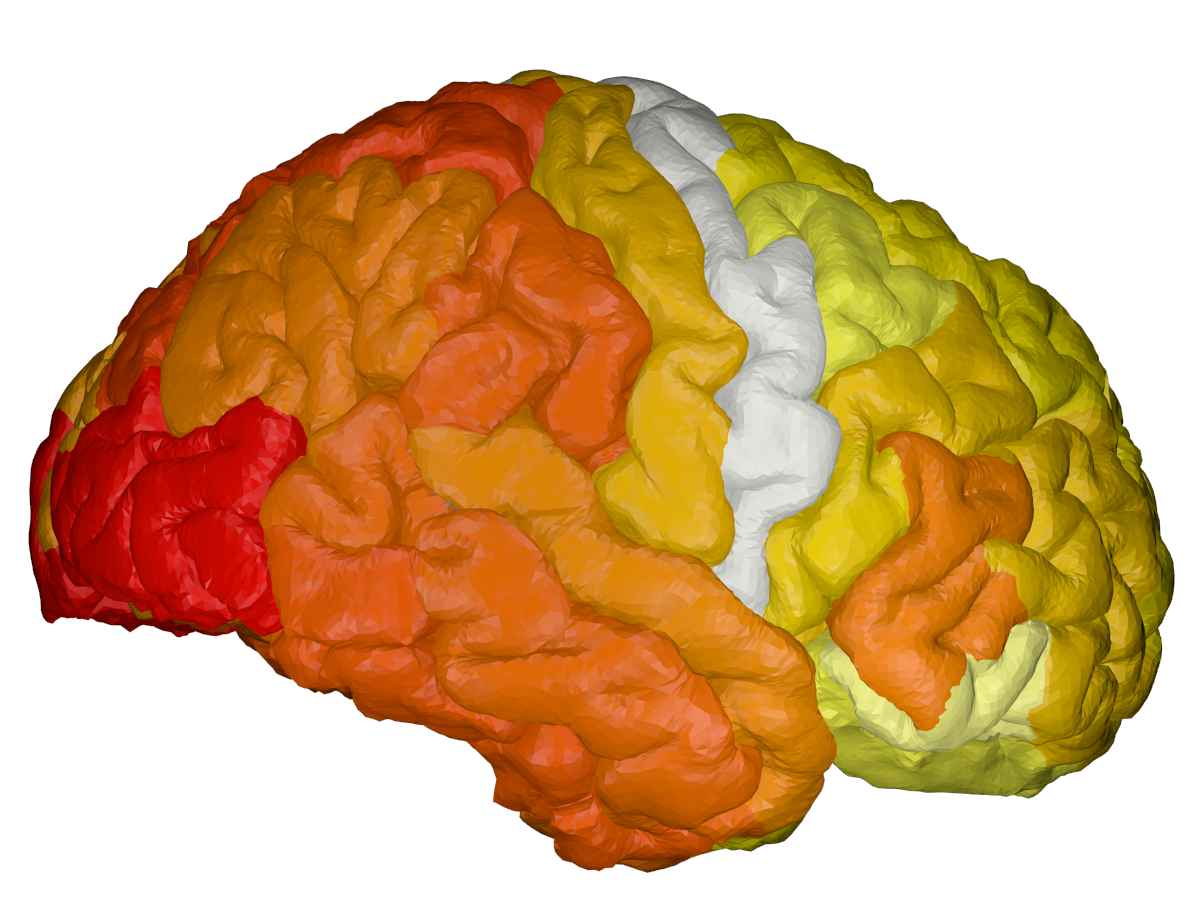
\includegraphics[height=1cm,trim=0 0 900 0]{images/brainTransparent} 
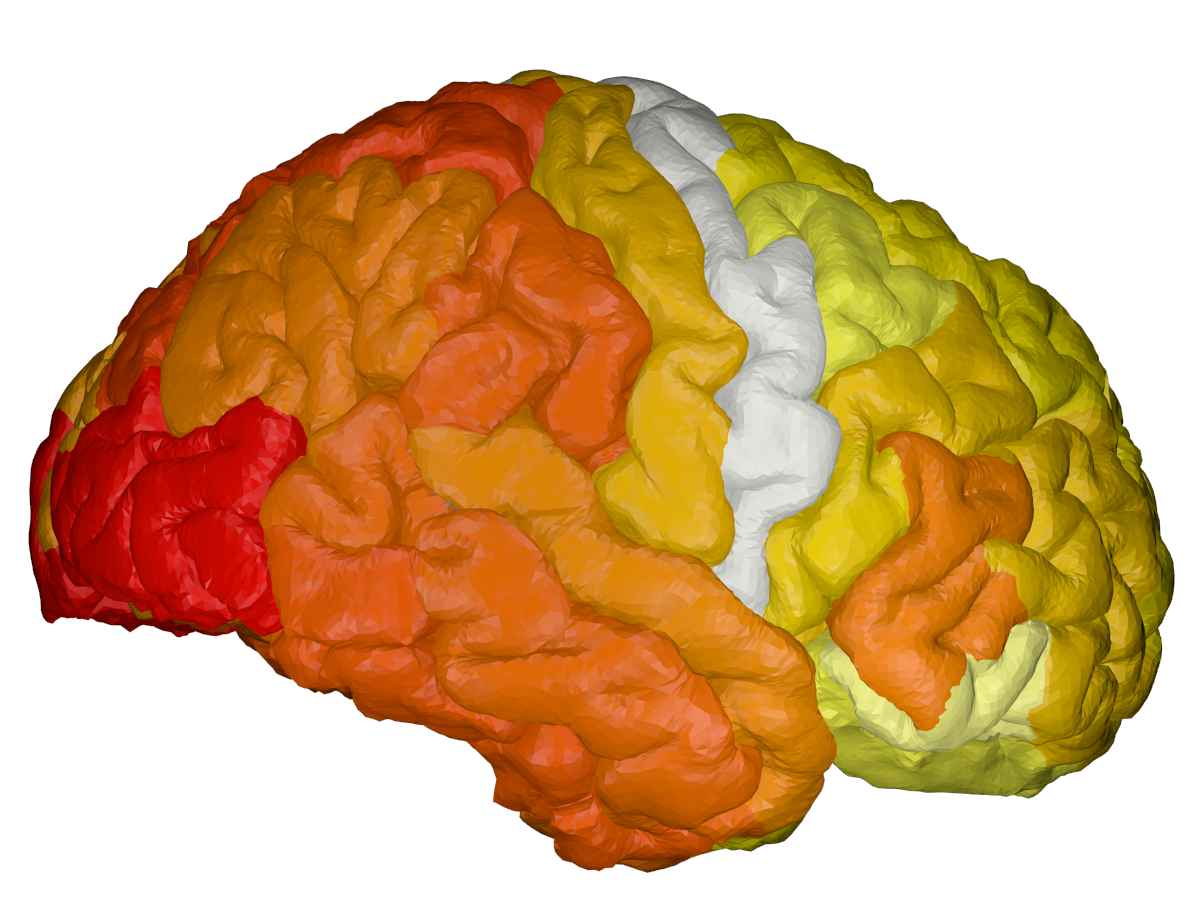
\includegraphics[height=1cm,trim=0 0 900 0]{images/brainTransparent} 
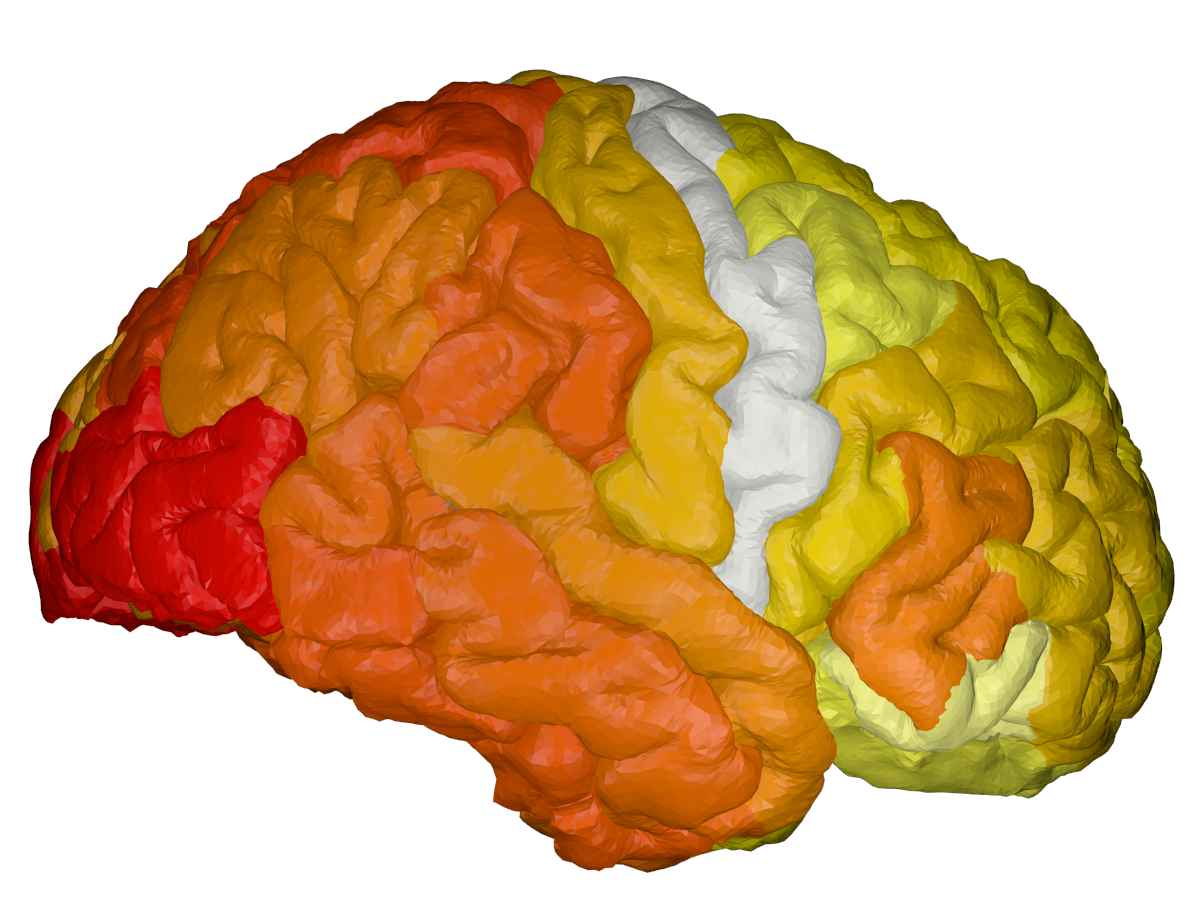
\includegraphics[height=1cm,trim=0 0 900 0]{images/brainTransparent} 
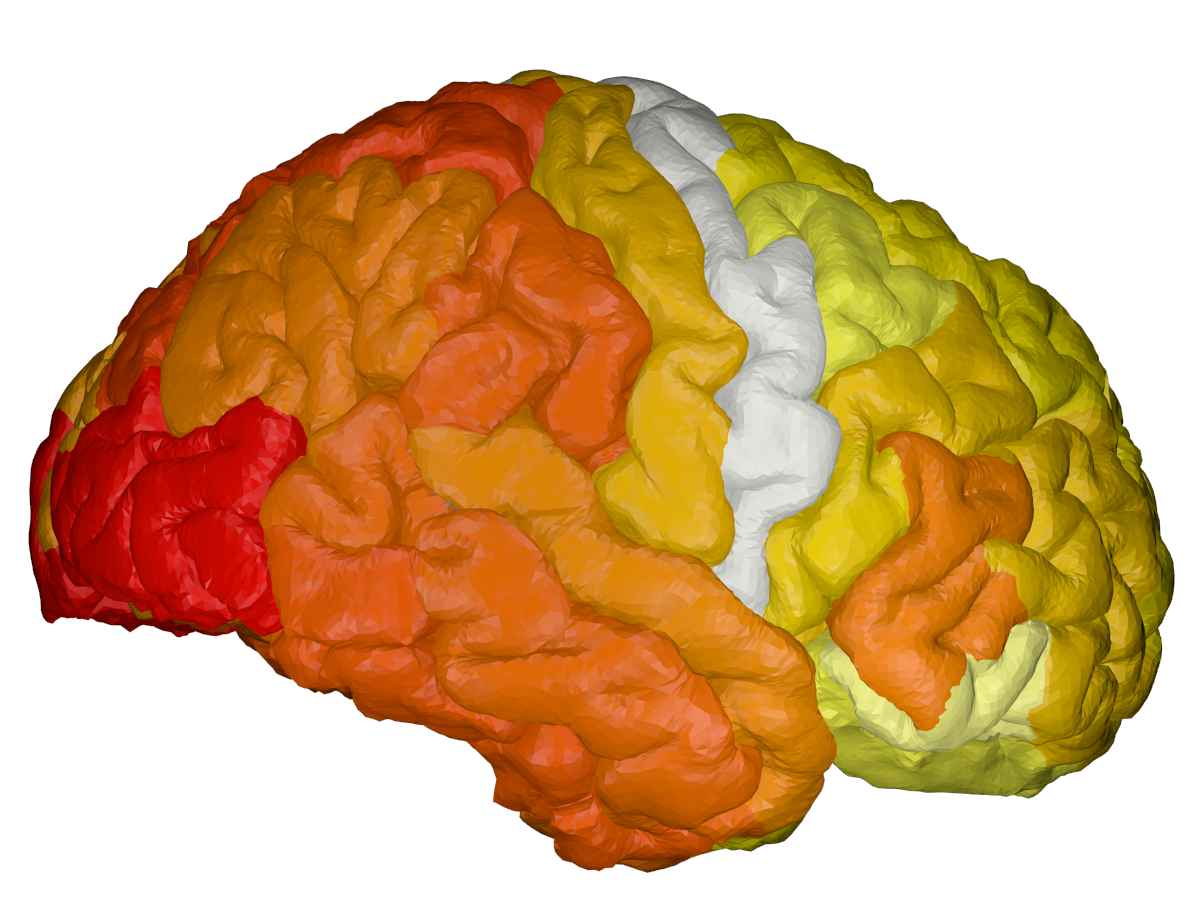
\includegraphics[height=1cm]{images/brainTransparent} 



\end{subfigure}
\begin{subfigure}[t]{0.3\textwidth}
\centering
 \begin{minipage}[t][3.5cm][t]{\textwidth}
 \centering
\myno volumetric images hard to visualise\\
\vspace{1.5em}
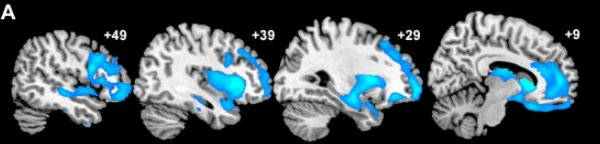
\includegraphics[width=\textwidth]{images/seeleyImages} 
\vspace{1.0em}
 \end{minipage}


\myyes brain surface easy to visualise\\
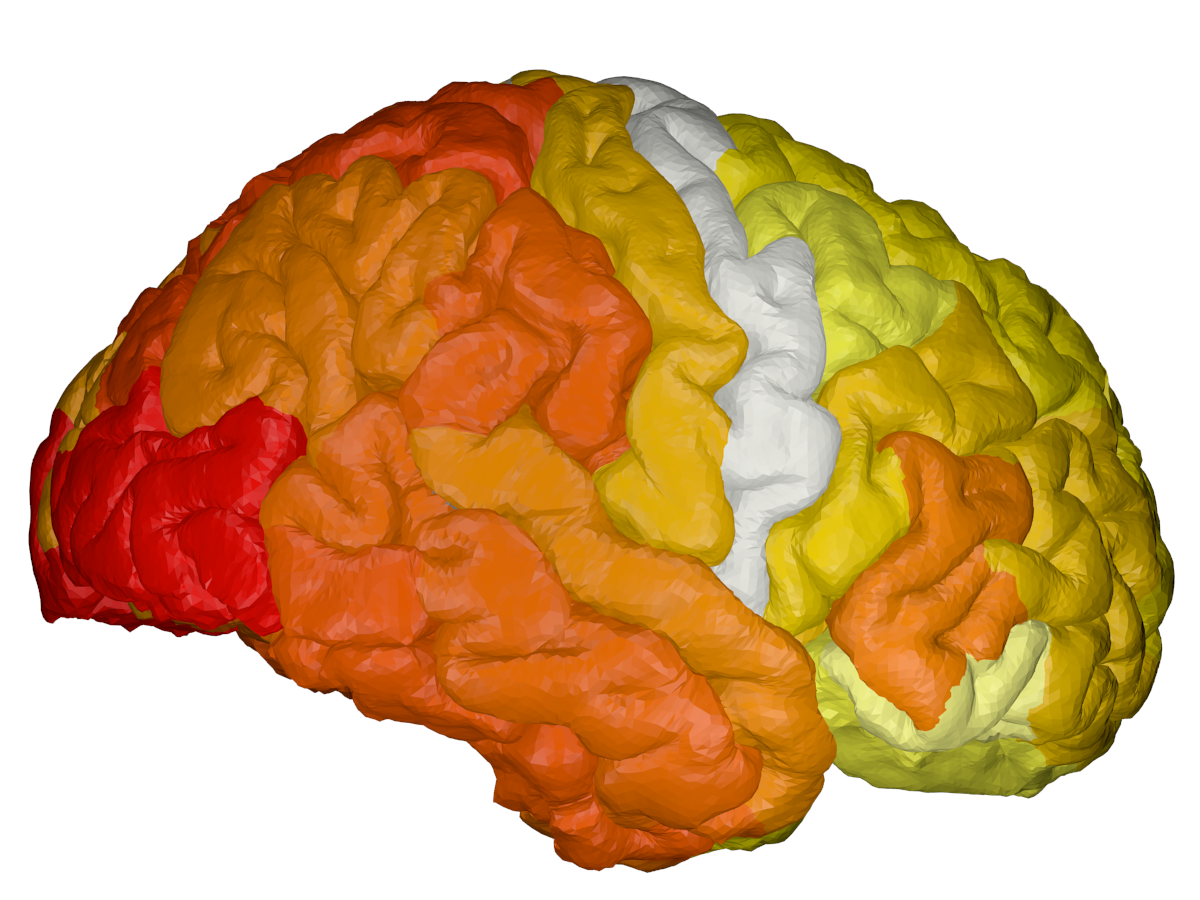
\includegraphics[width=0.5\textwidth]{images/cortical-outer_0} 


\end{subfigure}

\end{figure}
 
\end{frame}




\begin{frame}
 \frametitle{Further motivation}

 
\newcommand{\speed}{4} 
\newcommand{\animOne}{
\begin{animateinline}[autoplay,loop]{\speed}  
   \multiframe{24}{i=1+1}{% loop through pictures
%  \multiframe{1}{i=1+1}{% loop through pictures \multiframe{nrOfPics}{i=initialVal+increment} 
  \centering
   \includegraphics[width=0.25\textwidth]{images/sara_video/outer-\i.png}
  }
\end{animateinline}
}
 
\begin{itemize}
 \item simple input files $\rightarrow$ no need to read specifications and integrate with FreeSurfer, SPM, etc ..
 \item automated image generation $\rightarrow$ create movies showing e.g. progression of brain pathology

 
\begin{figure}
\begin{tikzpicture}

 \node (A) at (-3,0) {
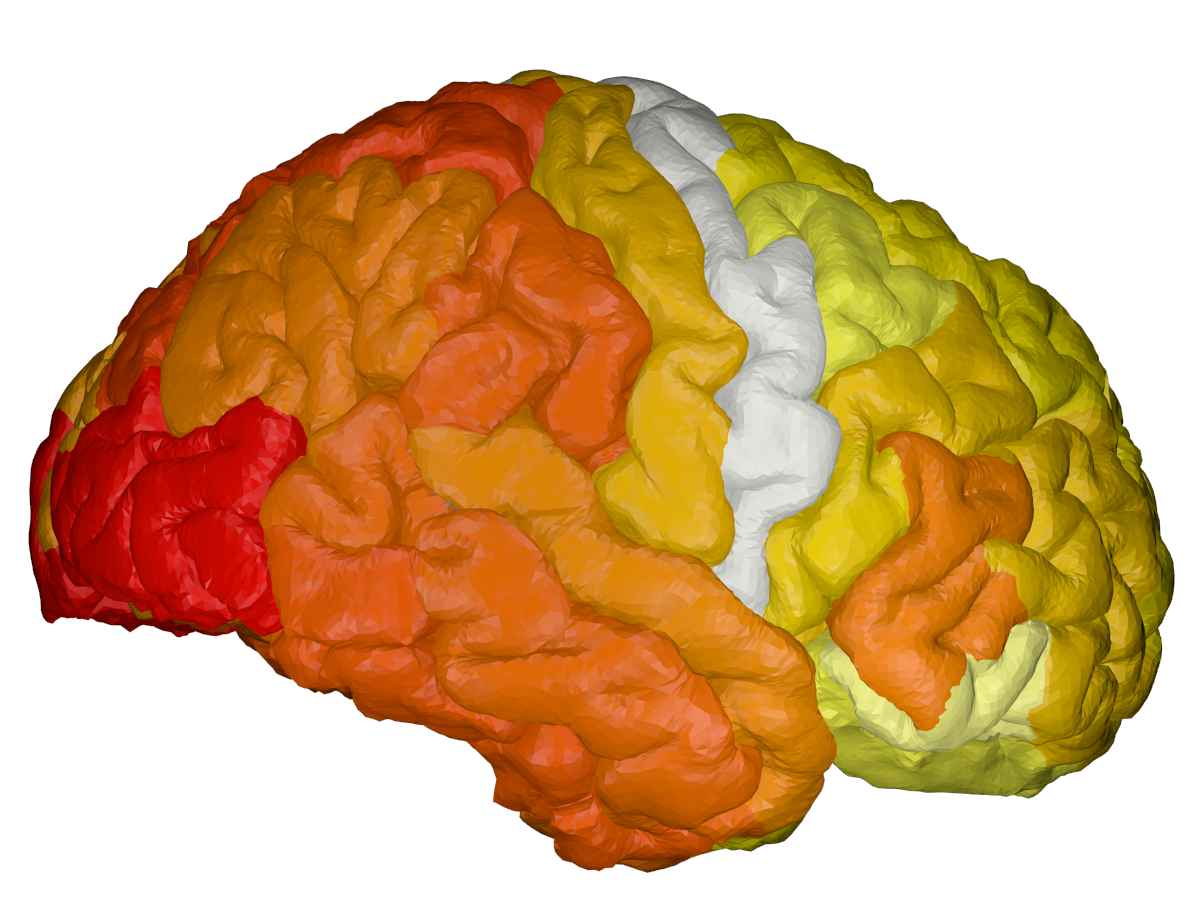
\includegraphics[height=2cm,trim=0 0 900 0]{images/brainTransparent} 
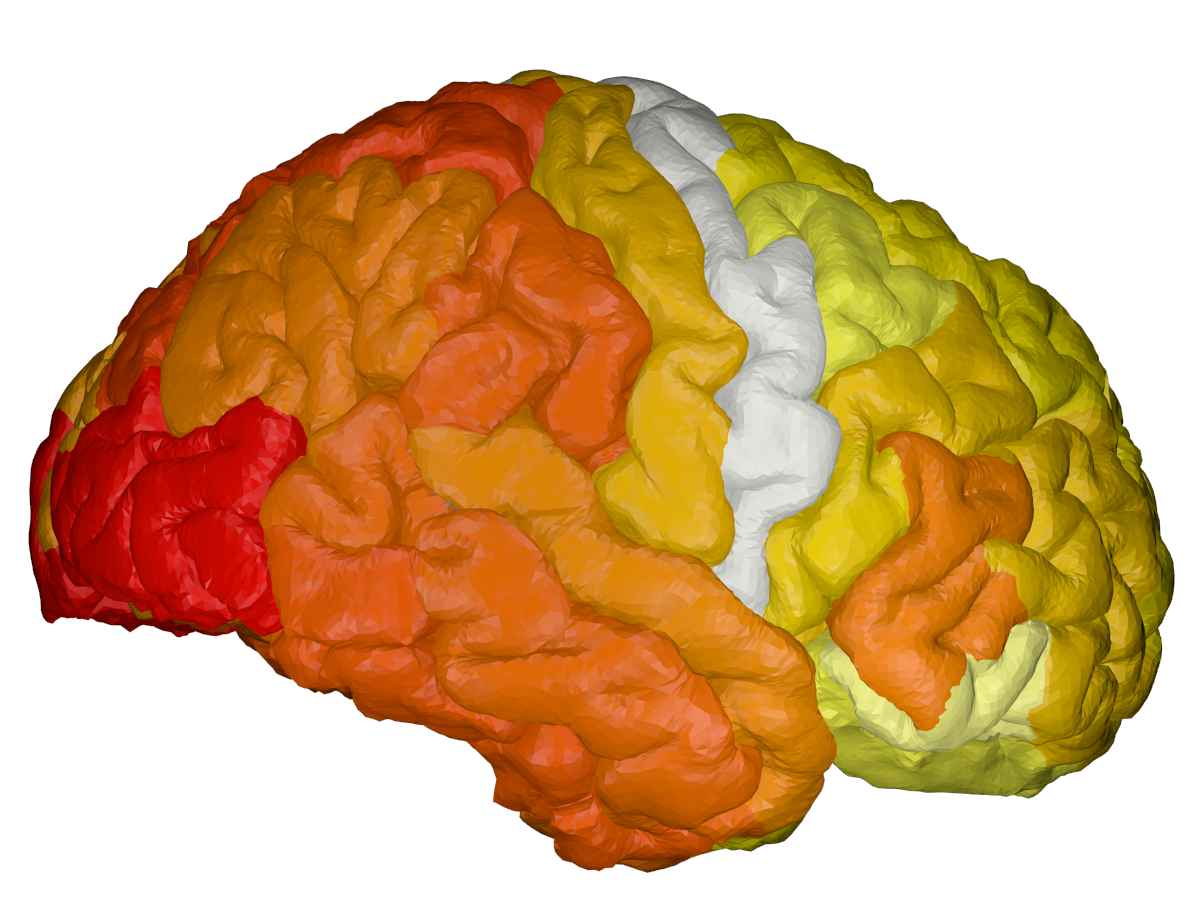
\includegraphics[height=2cm,trim=0 0 900 0]{images/brainTransparent} 
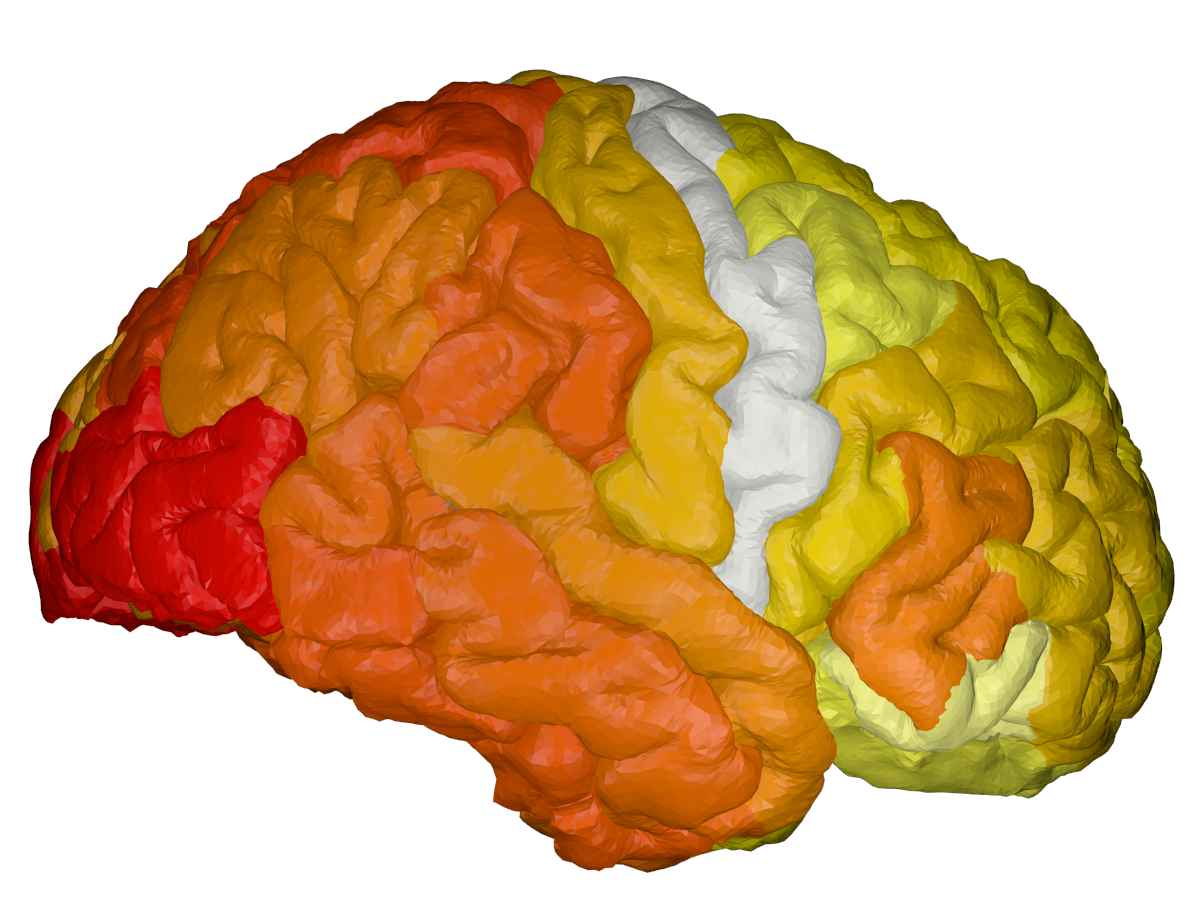
\includegraphics[height=2cm,trim=0 0 900 0]{images/brainTransparent} 
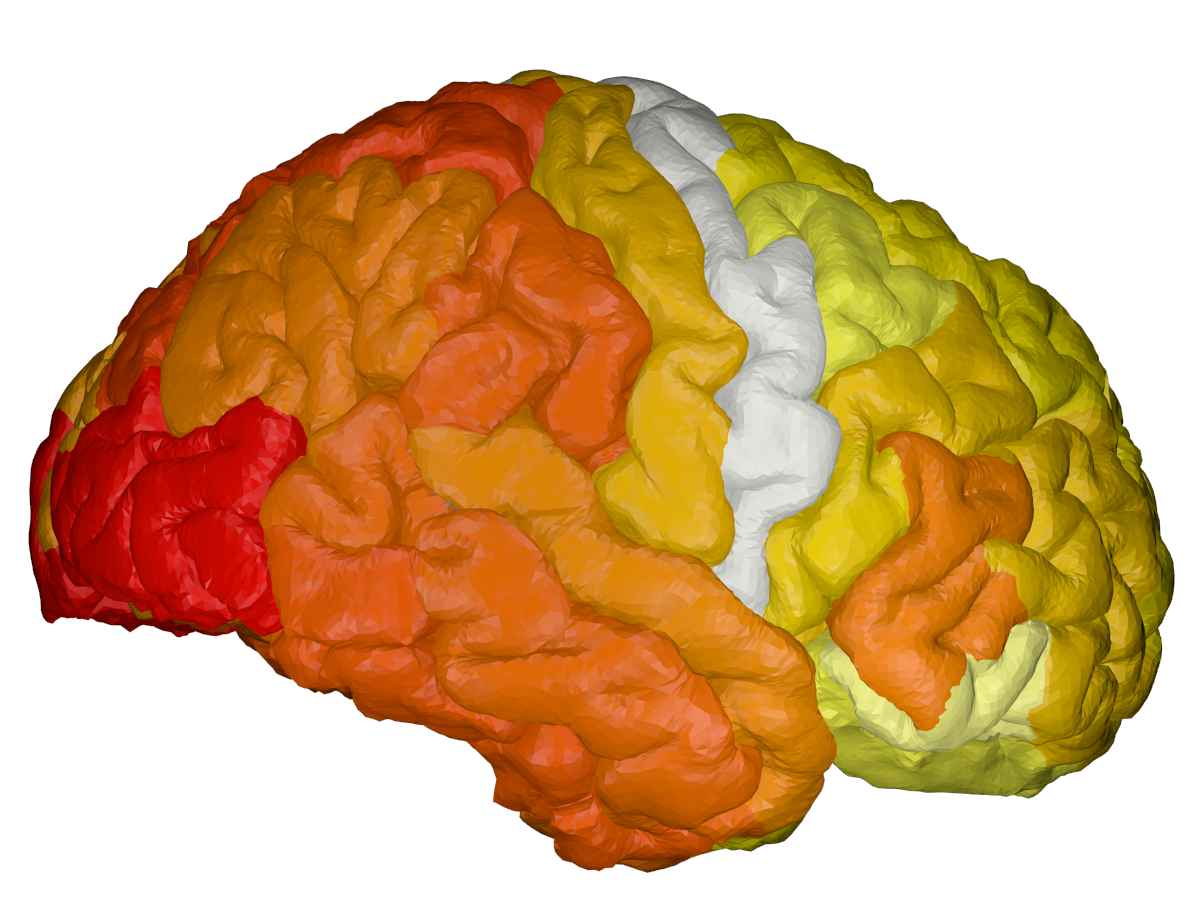
\includegraphics[height=2cm]{images/brainTransparent} 
};
 \node (B) at (3,0) {\animOne};

 \draw[thick,->] (A.east) -- (B.west);
  \end{tikzpicture}

\end{figure}
\end{itemize}

\vspace{-1em}

\begin{columns}
 \begin{column}{0.5\textwidth}
 \begin{itemize}
   \item surface representation $\rightarrow$ easy visualisation of subcortical structures 
   \begin{itemize}
     \item not possible in FreeSurfer
   \end{itemize}
 \end{itemize}
 \end{column}
\begin{column}{0.5\textwidth}
%   \begin{figure}
%   \centering
  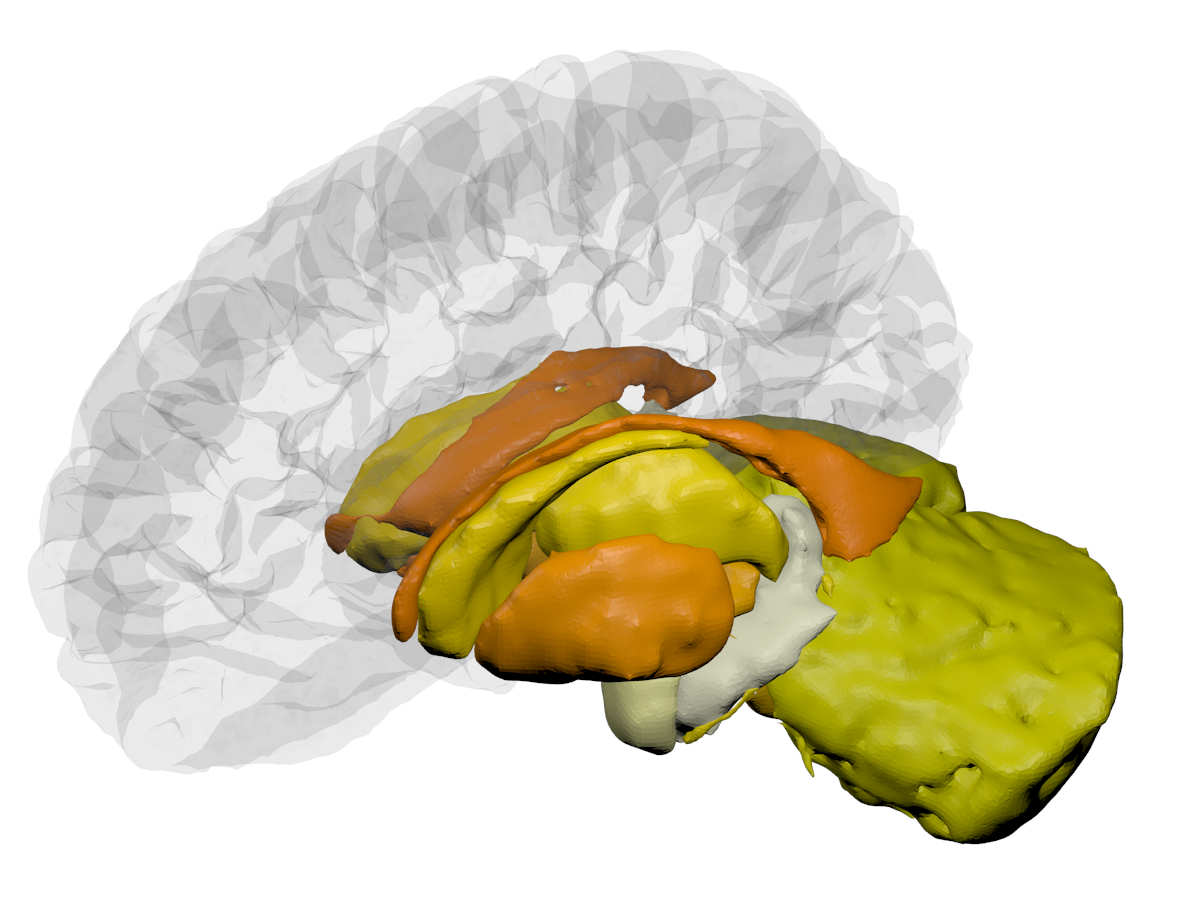
\includegraphics[height=3cm]{images/DK_output/Image_1_subcortical}
%  \end{figure}
\end{column}
\end{columns}
 
 
 
%  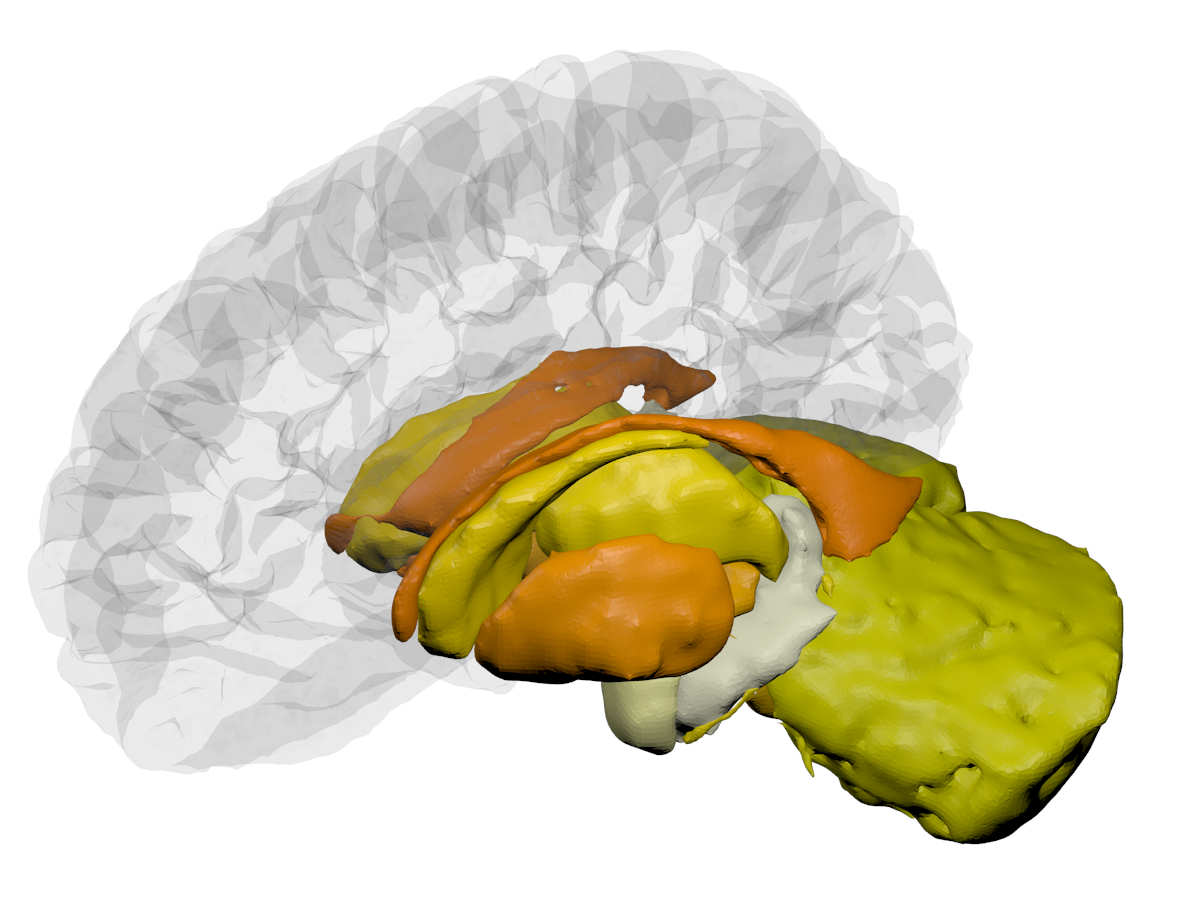
\includegraphics[height=2cm]{images/DK_output/Image_1_subcortical}
 
 
 
% 1. no need to integrate with Freesurfer, SPM, etc ... - Generic input data
% 2. creating movies showing e.g. progression of pathology
% 3. no need to show multiple slices due to surface visualisation
\end{frame}




\begin{frame}
 \frametitle{BrainPainter: How it works}

  
\begin{figure}
\centering
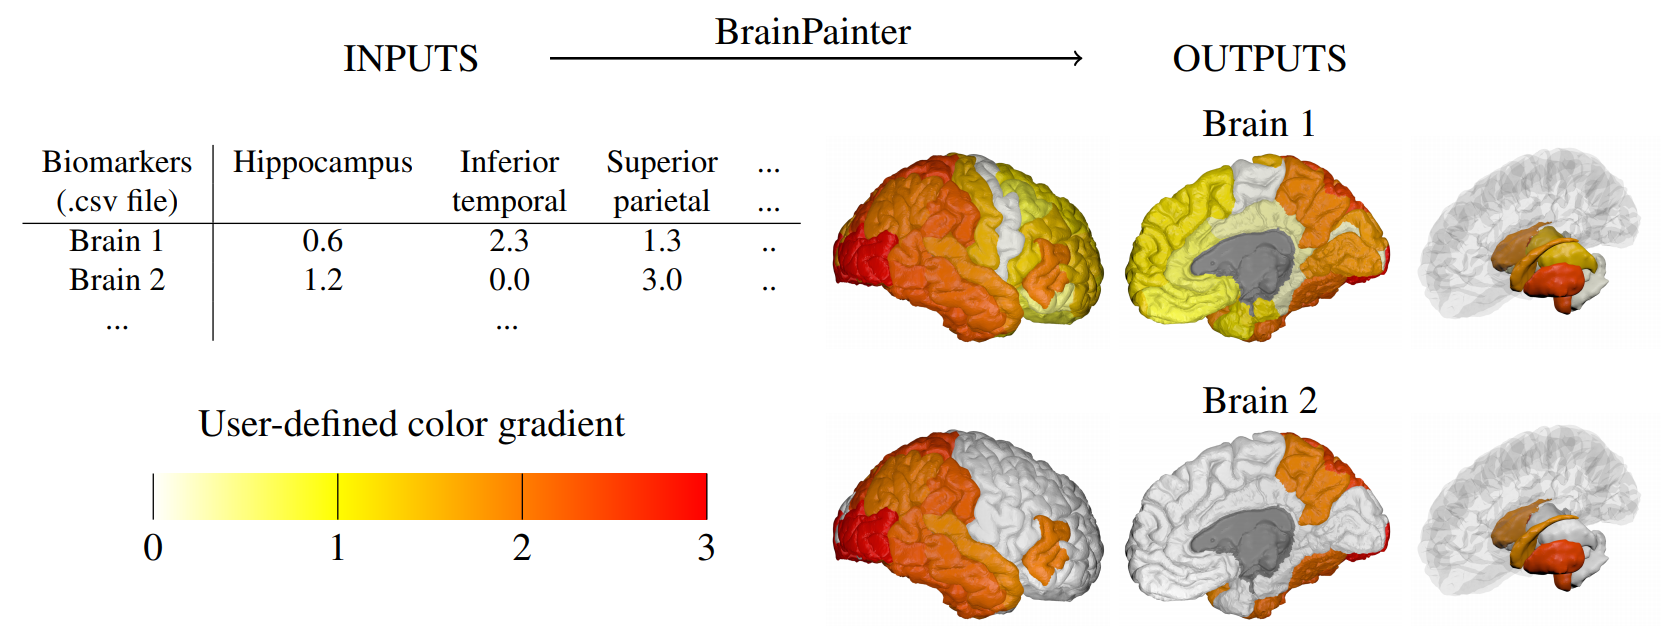
\includegraphics[height=5cm]{images/diagram.png}
\end{figure}
 
\begin{itemize}
 \item Uses Blender to generate images from pre-defined templates
\end{itemize}


 
\end{frame} 


\begin{frame}[t]{BrainPainter is customisable}

%  \begin{itemize}
%   \item Generates a brain visualisation from a list of numbers mapping to a color gradient
%   \item Customisable:


\begin{columns}[t]
\begin{column}{0.5\textwidth}


 \begin{itemize}
   \item supports three atlases:
   \begin{figure}
    \fontsize{8}{10}\selectfont
     \begin{subfigure}{0.27\textwidth}
      \centering
      Desikan-Killiany\\
      \includegraphics[height=1.5cm]{images/DK_output/Image_2_cortical-outer.png}
     \end{subfigure}
     \begin{subfigure}{0.27\textwidth}
      \centering
      Destrieux\\
      \includegraphics[height=1.5cm]{images/Destrieux_output/Image_2_cortical-outer.png}
     \end{subfigure}
     \begin{subfigure}{0.27\textwidth}
      \centering
      Tourville\\
      \includegraphics[height=1.5cm]{images/Tourville_output/Image_2_cortical-outer.png}
     \end{subfigure}

   \end{figure}
   
   \vspace{2em}
   
   \item supports different surfaces
   \begin{figure}
    \fontsize{8}{10}\selectfont
     \begin{subfigure}{0.27\textwidth}
      \centering
      pial\\
      \includegraphics[height=1.5cm]{images/DK_output/Image_2_cortical-outer.png}
     \end{subfigure}
     \begin{subfigure}{0.27\textwidth}
      \centering
      inflated\\
      \includegraphics[height=1.5cm]{images/DK_output_inflated/Image_2_cortical-outer.png}
     \end{subfigure}
     \begin{subfigure}{0.27\textwidth}
      \centering
      white matter\\
      \includegraphics[height=1.5cm]{images/DK_output_white/Image_2_cortical-outer.png}
     \end{subfigure}

   \end{figure}
   
   

\end{itemize}
 

\end{column}
\begin{column}{0.5\textwidth}  %%<--- here


 \begin{itemize}
   \item supports three pre-defined viewpoints
      \begin{figure}
    \fontsize{8}{10}\selectfont
     \begin{subfigure}{0.25\textwidth}
      \centering
      Outer Cortical\\
      \includegraphics[height=1.5cm]{images/DK_output/Image_2_cortical-outer.png}
     \end{subfigure}
     \begin{subfigure}{0.25\textwidth}
      \centering
      Inner Cortical\\
      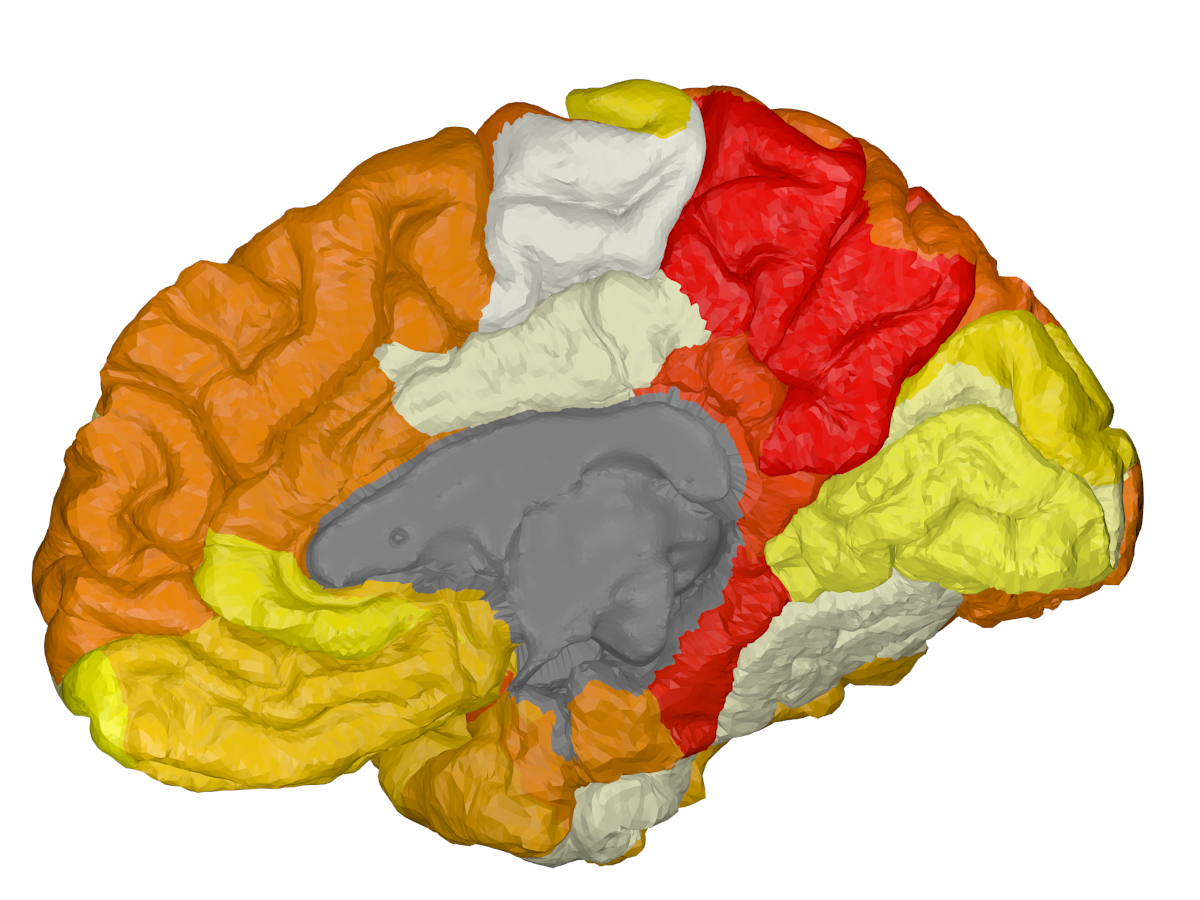
\includegraphics[height=1.5cm]{images/DK_output/Image_2_cortical-inner.png}
     \end{subfigure}
     \begin{subfigure}{0.25\textwidth}
      \centering
      Subcortical\\
      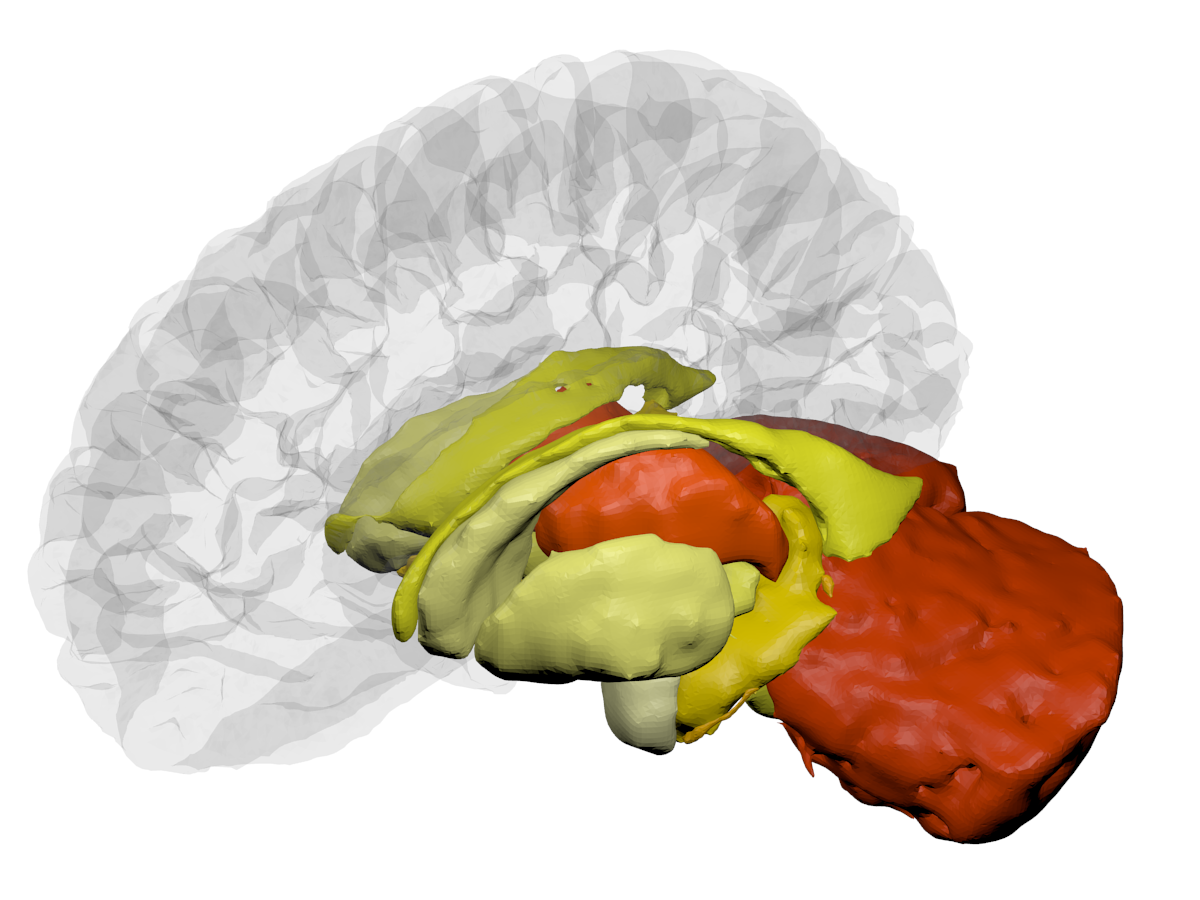
\includegraphics[height=1.5cm]{images/DK_output/Image_2_subcortical.png}
     \end{subfigure}

   \end{figure}
   
   \vspace{2em}
   
      
   
   \item user-defined colour gradient
   \item resolution
   \item background color
   \item ...
   
%    \item useful pre-defined settings instead of full customisation
   

  \end{itemize}



\end{column}
\end{columns}

  
% \end{itemize}

\end{frame}
 
\begin{frame}
 \frametitle{Example Use 1: Visualise degree of atrophy in Alzheimer's disease}
 
\begin{figure}
\centering
 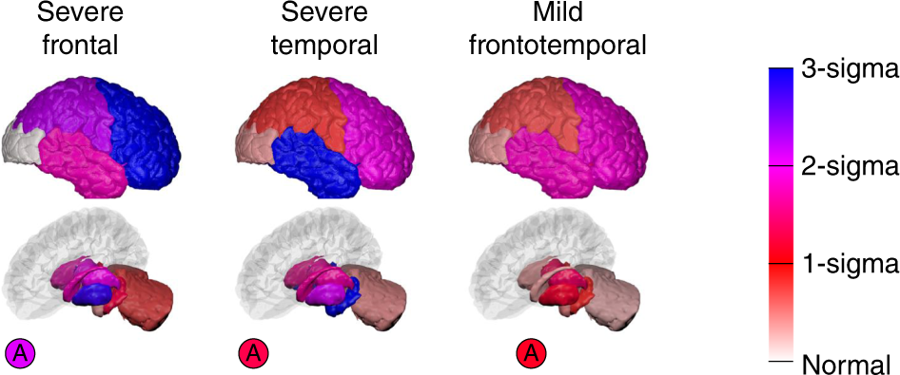
\includegraphics[width=0.5\textwidth]{images/young_3brains.png}
 
 Young et al, Nature Comms., 2018
\end{figure}
 
\end{frame}

\begin{frame}
 \frametitle{Example Use 2: Visualise temporal progression of atrophy in Alzheimer's subtypes}

 \begin{figure}
\centering
 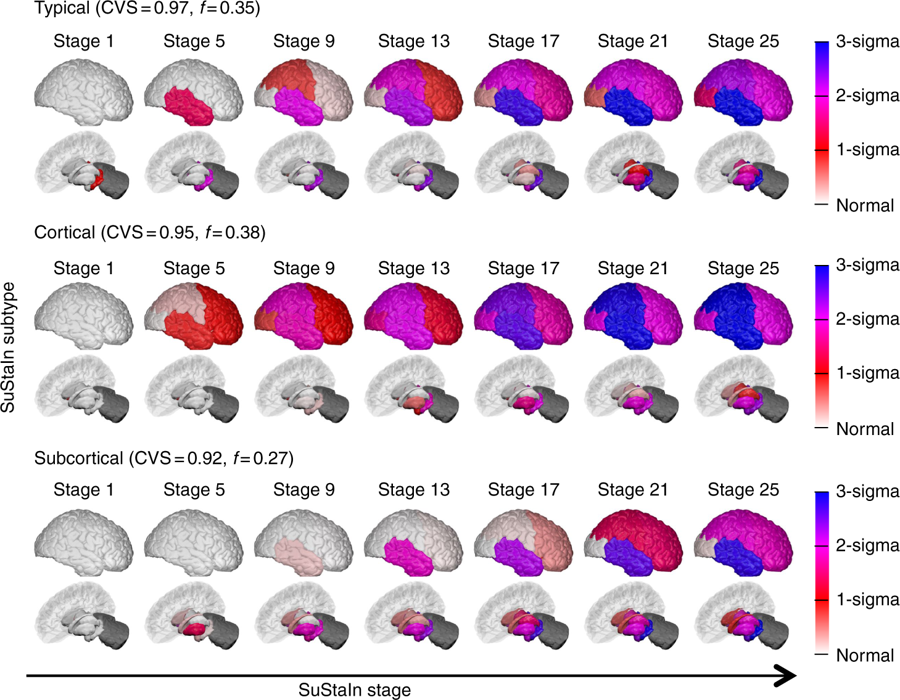
\includegraphics[width=0.5\textwidth]{images/young_progression.png}
 
 Young et al, Nature Comms., 2018
\end{figure}
 
\end{frame}

\begin{frame}
 \frametitle{Example Use 3: Visualise subcortical atrophy in Huntington's disease}
\begin{figure}[htp]
\centering
% \subfigure{Stage 0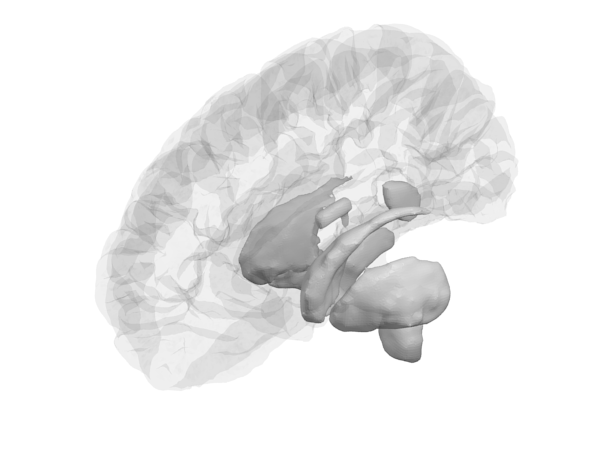
\includegraphics[width=0.2\textwidth]{images/ebmhd_pngs/subcortical_stage0.png}}
% \subfloat[Stage 0]{
\begin{subfigure}{0.2\textwidth}
\centering
No disease
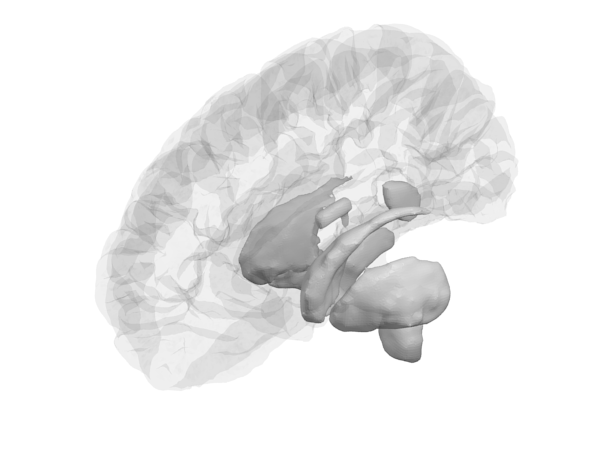
\includegraphics[width=1\textwidth,trim=70 0 70 0, clip]{images/ebmhd_pngs/subcortical_stage0.png}
\end{subfigure}
\begin{subfigure}{0.2\textwidth}
\centering
Early stage
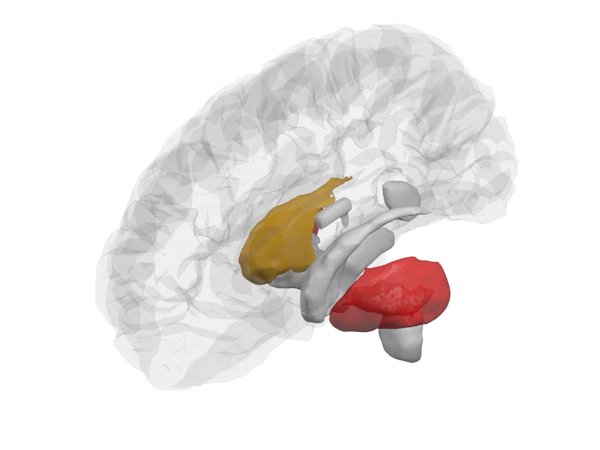
\includegraphics[width=1\textwidth,trim=70 0 70 0, clip]{images/ebmhd_pngs/subcortical_stage3.png}
\end{subfigure}
\begin{subfigure}{0.2\textwidth}
\centering
Middle stage
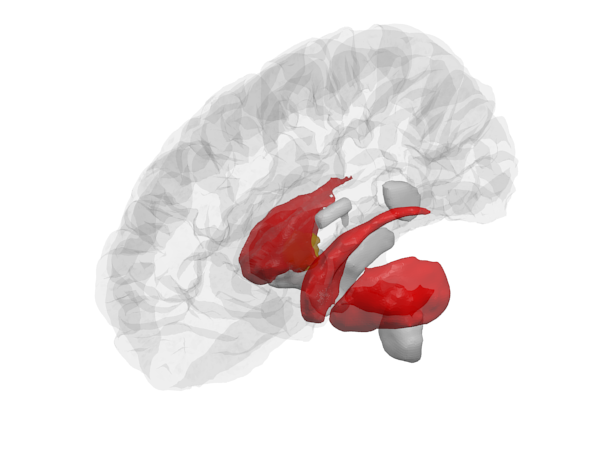
\includegraphics[width=1\textwidth,trim=70 0 70 0, clip]{images/ebmhd_pngs/subcortical_stage6.png}
\end{subfigure}
\begin{subfigure}{0.2\textwidth}
\centering
Late stage
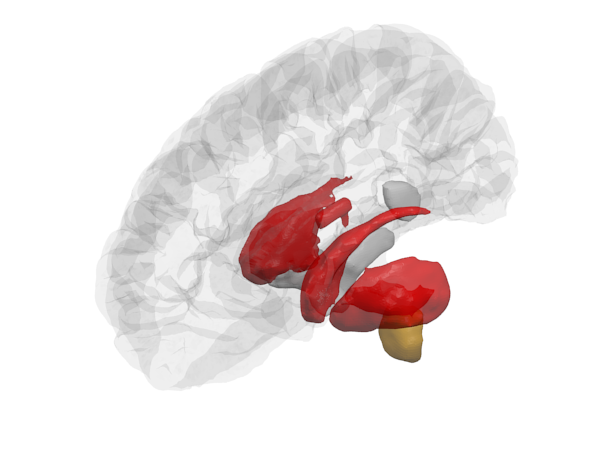
\includegraphics[width=1\textwidth,trim=70 0 70 0, clip]{images/ebmhd_pngs/subcortical_stage10.png}
\end{subfigure}\\
Wijeratne et al., Ann. Clin. Neurol., 2018
\end{figure}
 
\end{frame}

\begin{frame}
 \frametitle{Example Use 4: Animate the progression of amyloid spread in Alzheimer's disease}

 
\begin{figure}
\centering
\newcommand{\speed}{4} 
\begin{animateinline}[autoplay,loop]{\speed}  
    \multiframe{24}{i=1+1}{% loop through pictures
 % \multiframe{1}{i=1+1}{% loop through pictures \multiframe{nrOfPics}{i=initialVal+increment} 
  \parbox{\textwidth}{
  \centering
  \begin{subfigure}[b]{0.31\textwidth}
   \centering
   \includegraphics[width=\textwidth]{images/sara_video/outer-\i.png}
  \end{subfigure} 
  ~
  \begin{subfigure}[b]{0.31\textwidth}
   \centering
  \includegraphics[width=\textwidth]{images/sara_video/inner-\i.png}
  \end{subfigure}
  ~
  \begin{subfigure}[b]{0.31\textwidth}
   \centering
    \includegraphics[width=\textwidth]{images/sara_video/subcortical-\i.png} 
  \end{subfigure}
  }  
  }
\end{animateinline}

Garbarino and Lorenzi, IPMI, 2019
\end{figure}

  
\end{frame}


\begin{frame}
 \frametitle{BrainPainter runs straight from the browser - Live Demo}
 
 \begin{itemize}
  \item https://brainpainter.csail.mit.edu/
 
 \begin{figure}
  \includegraphics[width=0.6\textwidth]{images/frontPage}
 \end{figure}
 
 \item can also run from source: https://github.com/mrazvan22/brain-coloring
 \begin{itemize}
  \item requires no installation, run straight from docker container
 \end{itemize}
 
 \end{itemize}
 
  
\end{frame}


\begin{frame}
 \frametitle{Future work}

 \vspace{-2em}
 
 \begin{columns}
  \begin{column}[t]{0.5\textwidth}
  \begin{itemize}
  \item improve robustness of website, add error messages for wrong input
  
  \vspace{2em}
  
  \item support for other brain templates: e.g. infants, mice\\
  \vspace{1em}
  \includegraphics[height=2cm]{images/infantBrain} \includegraphics[height=2cm]{images/mouse}
    
   \end{itemize}
  \end{column}
  \begin{column}[t]{0.5\textwidth}

  \begin{itemize}
  \item more atlases: e.g. Hammers
  
  \vspace{3em}
  
  \item other visualisations: e.g. white-matter tracts\\
  \vspace{2em}
  
  \includegraphics[height=2cm]{images/wmTracts}

%    \item 
  \end{itemize}

  
  \end{column}

 \end{columns}

 
 
 
  
\end{frame}


\begin{frame}
 \frametitle{Acknowledgements}


% \begin{columns}
% \begin{column}{0.5\textwidth}

\textbf{Collaborators}
\begin{figure}
\begin{subfigure}{0.2\textwidth}
\centering
Polina Golland\\

\includegraphics[height=2cm]{images/polina} 
\end{subfigure}
\begin{subfigure}{0.2\textwidth}
\centering
Daniel Alexander
\includegraphics[height=2cm]{images/danny} 
\end{subfigure}
\begin{subfigure}{0.2\textwidth}
\centering
Arman Eshaghi\\
 
\includegraphics[height=2cm]{images/arman} 
\end{subfigure}
\begin{subfigure}{0.2\textwidth}
 \begin{itemize}
%   \item Polina Golland
%   \item Daniel Alexander
%   \item Arman Eshaghi
  \item Alexandra Young
  \item Sara Garbarino
  \item Peter Wijeratne
  \item ...
 \end{itemize}
\end{subfigure}



\end{figure}



% Collaborators:
\vspace{1em}

\textbf{Funders}\\
\begin{columns}
\begin{column}{0.4\textwidth}

\vspace{1em}

\includegraphics[height=2cm]{images/nac_logo} \hspace{2em}
\includegraphics[height=2cm]{images/epsrc_logo}
\end{column}
\begin{column}{0.4\textwidth}
% \vpsace{1em}
Anders Winkler for the 3D brain templates\\
 \begin{itemize}
  \item https://brainder.org/research/brain-for-blender/
 \end{itemize}

\end{column}

\end{columns}
 

 

  
\end{frame}


% \end{comment}

\end{document}



